\documentclass[12pt,dvipdfmx]{book}
\usepackage[margin=1in]{geometry}
\usepackage{amsmath,amssymb,amsfonts,mathtools,amsthm}
\usepackage[dvipdfmx]{graphicx}
\usepackage{tcolorbox,todonotes}
%\usepackage{slashbox}
%\usepackage{wrapfig}
%\usepackage{url,xspace,ascmac}
%\usepackage[]{xcolor}
%\usepackage{tcolorbox,todonotes}
\tcbuselibrary{breakable, skins, theorems}
%\usepackage{svg}
%\usepackage{etoolbox}
%\usepackage[subrefformat=parens]{subcaption}
%\usepackage{algorithm}
%\usepackage{algorithmic}
\usepackage[normalem]{ulem}
\usepackage{comment,tikz}
%\usepackage{todonotes}
%\usepackage{thmtools,thm-restate}
%\usepackage{enumitem}
%\usepackage{ifthen}
%\usepackage{float}

\usetikzlibrary{positioning,calc}

\tikzset{every picture/.style={font issue=\footnotesize},
            font issue/.style={execute at begin picture={#1\selectfont}}
        }

\usepackage[unicode,colorlinks=true,citecolor=blue,linkcolor=blue,pdfusetitle]{hyperref}
\usepackage[style=alphabetic,natbib=true,natbib=true,maxnames=99,maxalphanames=99,isbn=false,url=false,backref=true,backend=biber,giveninits=true]{biblatex}

%\usepackage[style=alphabetic,natbib=true,maxnames=99,maxalphanames=99]{biblatex}
\addbibresource{ref.bib}

\usepackage{cleveref}

\newcommand{\kara}{} %無を出力するコマンド

%def
\newtcolorbox[auto counter, number within=section, crefname = {定義}{定義}]{definition}[3][]
{enhanced, breakable = true, fonttitle = \bfseries,
title = 定義~\thetcbcounter~\if #2\kara \else(#2) \fi,
#1,
label = def:#3}

%thm
\newtcolorbox[auto counter, use counter from=definition, crefname = {定理}{定理}]{theorem}[3][]
{enhanced, colback = orange!10!white, colframe = red!50!black, breakable = true, fonttitle = \bfseries,
title = 定理~\thetcbcounter~\if #2\kara \else(#2) \fi,
#1,
label = thm:#3}

%prop
\newtcolorbox[auto counter, use counter from=definition, crefname = {命題}{命題}]{proposition}[3][]
{enhanced,  colback = orange!10!white, colframe = red!50!black, breakable = true, fonttitle = \bfseries,
title = 命題~\thetcbcounter~\if #2\kara \else(#2) \fi,
#1,
label = prop:#3}

%lemma
\newtcolorbox[auto counter, use counter from=definition, crefname = {補題}{補題}]{lemma}[3][]
{enhanced,  colback = green!10!white, colframe = green!50!black, breakable = true, fonttitle = \bfseries,
title = 補題~\thetcbcounter~\if #2\kara \else(#2) \fi,
#1,
label = lem:#3}

%cor
\newtcolorbox[auto counter, use counter from=definition, crefname = {系}{系}]{corollary}[3][]
{enhanced, breakable = true, fonttitle = \bfseries,
title = 系~\thetcbcounter~\if #2\kara \else(#2) \fi,
#1,
label = cor:#3}

%remark
\newtcolorbox[auto counter, use counter from=definition, crefname = {注釈}{注釈}]{remark}[3][]
{enhanced, breakable = true, colback = white, fonttitle = \bfseries,
title = 注釈~\thetcbcounter~\if #2\kara \else(#2) \fi,
#1,
label = rem:#3}

%exercise
\newtcolorbox[auto counter, crefname = {演習問題}{演習問題}]{exercise}[3][]
{enhanced, breakable = true, colback = blue!10!white, colframe = blue!50!black, fonttitle = \bfseries,
title = 演習問題~\thetcbcounter~\if #2\kara \else(#2) \fi,
#1,
label = exer:#3}

%example
\newtcolorbox[auto counter, use counter from=definition, crefname = {例}{例}]{example}[3][]
{enhanced, breakable = true, colback = brown!10!white, colframe = brown!50!black, fonttitle = \bfseries,
title = 例~\thetcbcounter~\if #2\kara \else(#2) \fi,
#1,
label = ex:#3}

%algorithm
\newtcolorbox[auto counter, use counter from=definition, crefname = {アルゴリズム}{アルゴリズム}]{algorithm}[3][]
{enhanced, breakable = true, colback = cyan!10!white, colframe = cyan!50!black, fonttitle = \bfseries,
title = アルゴリズム~\thetcbcounter~\if #2\kara \else(#2) \fi,
#1,
label = alg:#3}

%claim
\newtcolorbox[auto counter, use counter from=definition, crefname = {主張}{主張}]{claim}[3][]
{enhanced, breakable = true, colback = yellow!10!white, colframe = yellow!50!black, fonttitle = \bfseries,
title = 主張~\thetcbcounter~\if #2\kara \else(#2) \fi,
#1,
label = claim:#3}

\renewcommand{\proofname}{\textbf{証明}}
\renewcommand{\figurename}{図}
\crefname{equation}{式}{式}
\crefname{section}{セクション}{セクション}
\crefname{figure}{図}{図}
\newcommand{\defeq}{\mathrel{:=}}
\DeclarePairedDelimiter{\floor}{\lfloor}{\rfloor} % floor function
\DeclarePairedDelimiter{\ceil}{\lceil}{\rceil} % ceil function
\let\ip\undefined
\DeclarePairedDelimiter{\ip}{\langle}{\rangle} % inner product

\newcommand{\Ver}{\mathrm{Ver}}
\newcommand{\Maj}{\mathrm{Maj}}
\newcommand{\indicator}[1]{\mathbf{1}_{#1}}
\newcommand{\condition}{\;\middle\vert\;}
\newcommand{\tand}{\text{ and }}
\newcommand{\tor}{\text{ or }}
\newcommand{\tif}{\text{if }}
\newcommand{\totherwise}{\text{otherwise}}

\newcommand{\Bin}{\mathrm{Bin}}

\newcommand{\true}{\mathsf{true}}
\newcommand{\false}{\mathsf{false}}
\newcommand{\e}{\mathrm{e}}
\DeclareMathOperator*{\E}{\mathbb{E}}
\DeclareMathOperator*{\Var}{\mathbf{Var}}
\newcommand{\dtv}{d_{\mathrm{TV}}}
\newcommand{\F}{\mathbb{F}}
\newcommand{\diam}{\mathrm{diam}}
\newcommand{\Fq}{\mathbb{F}_q}
\newcommand{\dist}{\mathrm{dist}}
\newcommand{\Nat}{\mathbb{N}}
\newcommand{\Real}{\mathbb{R}}
\newcommand{\Int}{\mathbb{Z}}
\newcommand{\Comp}{\mathbb{C}}
\newcommand{\binset}{\{0,1\}}
\newcommand{\supp}{\mathsf{supp}}
\renewcommand{\emph}[1]{\textbf{#1}}
\newcommand{\allone}{\mathbf{1}}
\newcommand{\Cay}{\mathrm{Cay}}

\newcommand{\argmax}{\mathop{\mathrm{argmax}}}
\newcommand{\RW}{\mathsf{RW}}

\newcommand{\val}{\mathrm{val}}
\newcommand{\UNSAT}{\mathrm{UNSAT}}
\renewcommand{\epsilon}{\varepsilon}
\newcommand{\size}{\mathrm{size}}

\newcommand{\PRIMES}{\mathrm{Primes}}
\newcommand{\ThreeCOL}{\mathrm{3COL}}
\newcommand{\LinEq}{\mathrm{LinEQ}}
\newcommand{\QuadEQ}{\mathrm{QuadEq}}
\newcommand{\ThreeQuadEQ}{\mathrm{3-QuadEq}}

\newcommand{\RS}{\mathrm{RS}}
\newcommand{\RM}{\mathrm{RM}}
\newcommand{\Had}{\mathrm{Had}}
\newcommand{\restr}[1]{|_{#1}}

\newcommand{\calA}{\mathcal{A}}
\newcommand{\calB}{\mathcal{B}}
\newcommand{\calC}{\mathcal{C}}
\newcommand{\calD}{\mathcal{D}}
\newcommand{\calE}{\mathcal{E}}
\newcommand{\calF}{\mathcal{F}}
\newcommand{\calG}{\mathcal{G}}
\newcommand{\calH}{\mathcal{H}}
\newcommand{\calI}{\mathcal{I}}
\newcommand{\calJ}{\mathcal{J}}
\newcommand{\calK}{\mathcal{K}}
\newcommand{\calL}{\mathcal{L}}
\newcommand{\calM}{\mathcal{M}}
\newcommand{\calN}{\mathcal{N}}
\newcommand{\calO}{\mathcal{O}}
\newcommand{\calP}{\mathcal{P}}
\newcommand{\calQ}{\mathcal{Q}}
\newcommand{\calR}{\mathcal{R}}
\newcommand{\calS}{\mathcal{S}}
\newcommand{\calT}{\mathcal{T}}
\newcommand{\calU}{\mathcal{U}}
\newcommand{\calV}{\mathcal{V}}
\newcommand{\calW}{\mathcal{W}}
\newcommand{\calX}{\mathcal{X}}
\newcommand{\calY}{\mathcal{Y}}
\newcommand{\calZ}{\mathcal{Z}}

\newcommand{\bolda}{\boldsymbol{a}}
\newcommand{\boldb}{\boldsymbol{b}}
\newcommand{\boldc}{\boldsymbol{c}}
\newcommand{\boldd}{\boldsymbol{d}}
\newcommand{\bolde}{\boldsymbol{e}}
\newcommand{\boldf}{\boldsymbol{f}}
\newcommand{\boldg}{\boldsymbol{g}}
\newcommand{\boldh}{\boldsymbol{h}}
\newcommand{\boldi}{\boldsymbol{i}}
\newcommand{\boldj}{\boldsymbol{j}}
\newcommand{\boldk}{\boldsymbol{k}}
\newcommand{\boldl}{\boldsymbol{l}}
\newcommand{\boldm}{\boldsymbol{m}}
\newcommand{\boldn}{\boldsymbol{n}}
\newcommand{\boldo}{\boldsymbol{o}}
\newcommand{\boldp}{\boldsymbol{p}}
\newcommand{\boldq}{\boldsymbol{q}}
\newcommand{\boldr}{\boldsymbol{r}}
\newcommand{\bolds}{\boldsymbol{s}}
\newcommand{\boldt}{\boldsymbol{t}}
\newcommand{\boldu}{\boldsymbol{u}}
\newcommand{\boldv}{\boldsymbol{v}}
\newcommand{\boldw}{\boldsymbol{w}}
\newcommand{\boldx}{\boldsymbol{x}}
\newcommand{\boldy}{\boldsymbol{y}}
\newcommand{\boldz}{\boldsymbol{z}}

\newcommand{\boldA}{\boldsymbol{A}}
\newcommand{\boldB}{\boldsymbol{B}}
\newcommand{\boldC}{\boldsymbol{C}}
\newcommand{\boldD}{\boldsymbol{D}}
\newcommand{\boldE}{\boldsymbol{E}}
\newcommand{\boldF}{\boldsymbol{F}}
\newcommand{\boldG}{\boldsymbol{G}}
\newcommand{\boldH}{\boldsymbol{H}}
\newcommand{\boldI}{\boldsymbol{I}}
\newcommand{\boldJ}{\boldsymbol{J}}
\newcommand{\boldK}{\boldsymbol{K}}
\newcommand{\boldL}{\boldsymbol{L}}
\newcommand{\boldM}{\boldsymbol{M}}
\newcommand{\boldN}{\boldsymbol{N}}
\newcommand{\boldO}{\boldsymbol{O}}
\newcommand{\boldP}{\boldsymbol{P}}
\newcommand{\boldQ}{\boldsymbol{Q}}
\newcommand{\boldR}{\boldsymbol{R}}
\newcommand{\boldS}{\boldsymbol{S}}
\newcommand{\boldT}{\boldsymbol{T}}
\newcommand{\boldU}{\boldsymbol{U}}
\newcommand{\boldV}{\boldsymbol{V}}
\newcommand{\boldW}{\boldsymbol{W}}
\newcommand{\boldX}{\boldsymbol{X}}
\newcommand{\boldY}{\boldsymbol{Y}}
\newcommand{\boldZ}{\boldsymbol{Z}}

\newcommand{\veca}{\vec{a}}
\newcommand{\vecb}{\vec{b}}
\newcommand{\vecc}{\vec{c}}
\newcommand{\vecd}{\vec{d}}
\newcommand{\vece}{\vec{e}}
\newcommand{\vecf}{\vec{f}}
\newcommand{\vecg}{\vec{g}}
\newcommand{\vech}{\vec{h}}
\newcommand{\veci}{\vec{i}}
\newcommand{\vecj}{\vec{j}}
\newcommand{\veck}{\vec{k}}
\newcommand{\vecl}{\vec{l}}
\newcommand{\vecm}{\vec{m}}
\newcommand{\vecn}{\vec{n}}
\newcommand{\veco}{\vec{o}}
\newcommand{\vecp}{\vec{p}}
\newcommand{\vecq}{\vec{q}}
\newcommand{\vecr}{\vec{r}}
\newcommand{\vecs}{\vec{s}}
\newcommand{\vect}{\vec{t}}
\newcommand{\vecu}{\vec{u}}
\newcommand{\vecv}{\vec{v}}
\newcommand{\vecw}{\vec{w}}
\newcommand{\vecx}{\vec{x}}
\newcommand{\vecy}{\vec{y}}
\newcommand{\vecz}{\vec{z}}

\newcommand{\bara}{\overline{a}}
\newcommand{\barb}{\overline{b}}
\newcommand{\barc}{\overline{c}}
\newcommand{\bard}{\overline{d}}
\newcommand{\bare}{\overline{e}}
\newcommand{\barf}{\overline{f}}
\newcommand{\barg}{\overline{g}}
\newcommand{\barh}{\overline{h}}
\newcommand{\bari}{\overline{i}}
\newcommand{\barj}{\overline{j}}
\newcommand{\bark}{\overline{k}}
\newcommand{\barl}{\overline{l}}
\newcommand{\barm}{\overline{m}}
\newcommand{\barn}{\overline{n}}
\newcommand{\baro}{\overline{o}}
\newcommand{\barp}{\overline{p}}
\newcommand{\barq}{\overline{q}}
\newcommand{\barr}{\overline{r}}
\newcommand{\bars}{\overline{s}}
\newcommand{\bart}{\overline{t}}
\newcommand{\baru}{\overline{u}}
\newcommand{\barv}{\overline{v}}
\newcommand{\barw}{\overline{w}}
\newcommand{\barx}{\overline{x}}
\newcommand{\bary}{\overline{y}}
\newcommand{\barz}{\overline{z}}

\newcommand{\boldalpha}{\boldsymbol{\alpha}}
\newcommand{\boldbeta}{\boldsymbol{\beta}}
\newcommand{\boldgamma}{\boldsymbol{\gamma}}
\newcommand{\bolddelta}{\boldsymbol{\delta}}
\newcommand{\boldepsilon}{\boldsymbol{\epsilon}}
\newcommand{\boldzeta}{\boldsymbol{\zeta}}
\newcommand{\boldeta}{\boldsymbol{\eta}}
\newcommand{\boldtheta}{\boldsymbol{\theta}}
\newcommand{\boldiota}{\boldsymbol{\iota}}
\newcommand{\boldkappa}{\boldsymbol{\kappa}}
\newcommand{\boldlambda}{\boldsymbol{\lambda}}
\newcommand{\boldmu}{\boldsymbol{\mu}}
\newcommand{\boldnu}{\boldsymbol{\nu}}
\newcommand{\boldxi}{\boldsymbol{\xi}}
\newcommand{\boldpi}{\boldsymbol{\pi}}
\newcommand{\boldrho}{\boldsymbol{\rho}}
\newcommand{\boldsigma}{\boldsymbol{\sigma}}
\newcommand{\boldtau}{\boldsymbol{\tau}}
\newcommand{\boldupsilon}{\boldsymbol{\upsilon}}
\newcommand{\boldphi}{\boldsymbol{\phi}}
\newcommand{\boldchi}{\boldsymbol{\chi}}
\newcommand{\boldpsi}{\boldsymbol{\psi}}
\newcommand{\boldomega}{\boldsymbol{\omega}}
\newcommand{\boldvarepsilon}{\boldsymbol{\varepsilon}}
\newcommand{\boldvartheta}{\boldsymbol{\vartheta}}
\newcommand{\boldvarrho}{\boldsymbol{\varrho}}
\newcommand{\boldvarsigma}{\boldsymbol{\varsigma}}
\newcommand{\boldvarphi}{\boldsymbol{\varphi}}
\newcommand{\boldvarpi}{\boldsymbol{\varpi}}

\newcommand{\varx}{\mathrm{x}}
\newcommand{\vary}{\mathrm{y}}

\title{PCP定理とその証明}
\author{清水 伸高 (東京科学大学)}
\date{}
\begin{document}
\maketitle
\tableofcontents
\chapter*{序文}



このノートは, 京都大学大学院理学研究科数学・数理解析専攻数理解析系で開催される集中講義「PCP定理の証明と応用」の講義ノートである.
計算量(computational complexity)とは, 問題を解くために必要な計算リソースの量(例えば計算時間, 記憶領域のサイズ, 乱択や量子性の有無や量)を意味し, 計算量理論(computational complexity theory)とはそれぞれの問題の計算量を明らかにするための理論である.
PCP定理とは, 判定問題(YesかNoで答える問題)の検証に要する計算量に関する結果であり,
端的に言うと, ある命題が真であると主張する証明が文字列として与えられたとき,
その証明を検証するためには, 通常, 全ての文字を見て確認する必要があるが,
PCP定理によれば, その証明の一部だけを見ることで, その命題が真であるか否かを確率的に検証することができるという驚くべき結果である.
例えば, ある実行列$A$と実ベクトル$b$に対して線形方程式系$Ax=b$は解を持つ, という命題を考えてみよう.
この命題が真であるならば実際に解の一つ$x$を証明として提示することができるが, その証明が正しいかどうかを検証するためには検証者は$Ax$を実際に計算し, その各成分が$b$と一致するかを確認する必要がある.
ところがPCP定理によれば, 巧妙に構成された証明$\pi$を提示することにより, その証明$\pi$全ての文字を見ることなく, 99\%の確率で正しく検証できるのである (ここでは確率的な検証, つまり検証者はランダムネスを用いた検証を行う設定を考える).

このように, 局所的な情報だけを使って全体の構造を推測できるというPCP定理の性質は, 単に理論的に興味深いだけでなく, 誤り訂正符号の構成, 確率論的手法の脱乱択化, 最適化問題の近似率限界の導出など, 理論計算機科学において広大な応用を持ち, 現在でも計算量理論の中心的な研究対象の一つである.
このような重要性を持つにもかかわらず, PCP定理の証明に包括的に日本語でアクセスできる文献は(筆者が知る限り本資料の執筆時点では)存在しない.
本講義ではPCP定理の証明を与えるとともに, その証明に用いられた計算量理論の基本的な概念や技法を解説し,
PCP定理の応用についても触れる.
僭越ながらもこれはPCP定理の証明に日本語でアクセスする(おそらく国内初の)資料であるといえる.
今回のような挑戦的な機会を与えてくださった河村彰星先生に感謝を申し上げる.

\addcontentsline{toc}{chapter}{Preface}
\chapter{導入}

この集中講義ではPCP定理と呼ばれる計算量理論の基本的な結果について解説し, その証明を与える.
PCP定理は1998年に\citet{AroraS98,AroraLMSS98}によって証明された.
この証明は代数的な手法に基づく誤り訂正符号を技巧的に組合せたものであり, 難解なものであったが, その後\citet{Din07}によってより簡潔な証明が与えられた.
この講義では\citet{Din07}による比較的簡単な証明を紹介する.
ちなみにDinurはのちにこの業績によりゲーデル賞を受賞している.

\section{検証能力}
\subsection{クラスNP}
\subsection{クラスAM}
\subsection{クラスPCP}

\section{PCP定理}

\subsection{自明な例}

\begin{theorem}{PCP定理}{PCPtheorem}
  ...
\end{theorem}


\section{制約充足問題(CSP)}
\subsection{充足可能性判定問題(SAT)}
\chapter{制約充足問題} \label{chap:CSP}
制約充足問題(Constraint Satisfaction Problem, CSP)は, 計算量理論において重要な問題の一つであり, PCP定理の証明においても中心的な役割を果たす.

\section{制約充足問題の定義}
制約充足問題とは端的に言えば連立方程式の解の存在性判定を問う判定問題である.

\begin{definition}{制約充足問題}{CSP}
\emph{制約充足問題(CSP)}とは次の要素からなる組$\varphi = (X,\Sigma,\calI,\calC)$を入力とする判定問題である:
\begin{itemize}
  \item \emph{アルファベット}: 有限集合$\Sigma$.
  \item \emph{変数列}: $X=(\varx_1,\dots,\varx_n)$.
  \item 制約の引数の列: $\calI=(I_1,\dots,I_m)$. ここで, 各$I_i$は $I_i\ne\emptyset$ かつ $I_i\subseteq [n]$を満たす.
  \item \emph{制約の列}: $\calC=(c_I)_{I\in\calI}$. ここで, 各$c_I$は$c_I \subseteq \Sigma^{\abs{I}}$を満たす.
\end{itemize}
各$\varx\in X$を\emph{変数}, 各$c_I\in\calC$を\emph{制約}という.

入力$(X,\Sigma,\calI,\calC)$は,
ある変数への割り当て$a \colon X \to \Sigma$が存在して, 任意の$I=\{i_1,\dots,i_k\}\in\calI$ (ただし$i_1<\dots<i_k$)について,
\begin{align*}
  a(I) := (a(\varx_{i_1}),\dots,a(\varx_{i_k})) \in c_I
\end{align*}
であるとき, かつその時に限りYesインスタンスである.

全ての$i\in[m]$について$\abs{I_i}\le q$であるとき, このCSPは\emph{$q$-CSP}という.

また, 固定した割り当て$a \colon X\to \Sigma$に対する$\varphi$の\emph{不満足値}を
\begin{align*}
  \UNSAT_\varphi(a) = \Pr_{I\sim\calI}\qty[a(I) \not\in c_I]
\end{align*}
とする. ここで$I\sim\calI$は$I$が$\calI$から一様ランダムに選ばれたことを意味する.
さらに, 全ての割り当てに関して不満足値の最小値
\begin{align*}
  \UNSAT(\varphi) = \min_{a\in\Sigma^X} \UNSAT_\varphi(a)
\end{align*}
を$\varphi$の\emph{不満足値}という.
\end{definition}

各制約$c_I\in \calC$は, その制約が充足される割り当ての集合を表す.
例えば$c_I = \Sigma^{\abs{I}}$であるならば, 任意の割り当てに対して$c_I$は充足されるし,
$c_I = \emptyset$であるならば, どの割り当ても$c_I$を充足しない.

\begin{example}{グラフ彩色問題}{graph-coloring-problem-CSP}
  グラフ彩色問題(\cref{ex:graph-coloring-problem})は$2$-CSPである.
  実際, グラフ$G=(V,E)$に対して
  \begin{itemize}
    \item 変数列を$X=V$とする.
    \item アルファベットを$\Sigma=[k]$とする.
    \item 各制約$c_e$は各辺$e=\{u,v\}\in E$に付随していて,
    \begin{align*}
      (a_u,a_v) \in c_e \iff a_u\ne a_v
    \end{align*}
  と定義する.
  \end{itemize}
  このとき, グラフ$G$が$k$-彩色可能であることと, このCSPがYesインスタンスであることは同値である.
\end{example}




\subsection{PCPとの関係}
ランダムシード長$r=r(n)$かつクエリ数$q=O(1)$のPCP検証者は$\Sigma=\{0,1\}$の場合の$q$-CSPによって表現でき, 逆に$q$-CSPはPCP検証者として表現できる.
実際, $q$クエリのPCP検証者$V^\pi(x)$を考えよう.
証明の長さを$\abs{\pi}=\ell$とする.
入力$x$とランダムシード$s$を固定したときの$V^\pi(x;s)$が
証明中の読み込む文字のインデックスの集合を$I_s\subseteq[\ell]$とする (ここで$\abs{I_s}\le q$).
このとき, $V^\pi(x;s)$は$\binset^{I_s}$を$\binset$に写す関数を定める.
この関数を制約$c_s$とみなすことで, 検証者$V^\pi(x)$は$q$-CSPのインスタンスとして表現できる.
このとき, $q$-CSPのインスタンスの変数集合は証明$\pi$に対応する.
もし$x\in L$であるならば, 確率$1$で$V^\pi(x)=1$となるような$\pi$が存在する.
つまり, 全てのランダムシード$s$に対して$V^\pi(x;s)=1$となるような$\pi$が存在するため,
先ほど構成した$q$-CSPのインスタンスはYesインスタンスである.
逆に$x\not\in L$であるならば, 全ての$\pi$に対して確率$1/3$以上で$V^\pi(x)=0$となる.
これは, $q$-CSPインスタンスに対して, 全ての割り当てを考えても, 全体の制約のうち少なくとも$1/3$の割合は充足されない(すなわち, $\UNSAT$の値が$1/3$以上となる)ことを意味する.


\begin{table}[htbp]
  \centering
  \begin{tabular}{|c|c|}
    \hline
    PCP検証者 & $q$-CSP \\
    \hline
    PCP $\pi$ & 割り当て \\
    \hline
    ランダムネスを固定した時の判定 & CSPの制約 \\
    \hline
    PCP$\pi$を拒否する確率 & 割り当ての不満足値 $\UNSAT(\pi)$ \\
    \hline
  \end{tabular}
  \caption{PCPとCSPの対応関係}
  \label{table:pcp-csp-correspondence}
\end{table}

この対応関係に基づいて, PCP定理をCSPを用いた言葉で表すことができる.

\begin{theorem}{PCP定理のCSP版}{PCP-CSP-theorem}
  ある関数$m=n^{O(1)}$, $q=O(1)$, $\ell=n^{O(1)}$, 定数$c\in\Nat$, $\epsilon>0$, および
  次の性質を満たす多項式時間決定的アルゴリズム$A$が存在する:
  3彩色問題のインスタンス$G=(V,E)$を入力として受け取り, $G$の頂点数を$n$としたとき, $A$は高々$\ell(n)$個の変数と$m(n)$個の制約および要素数$c$のアルファベットからなる$q$-CSPのインスタンス$\varphi$を出力する.
  さらにこのインスタンス$\varphi$は
  \begin{itemize}
  \item 入力$G$が$\ThreeCOL$のYesインスタンスであるとき, $\UNSAT(\varphi) = 0$となる (すなわち$\varphi$はYesインスタンス).
  \item 入力$G$が$\ThreeCOL$のNoインスタンスであるとき, $\UNSAT(\varphi) \ge \epsilon$となる.
  \end{itemize}
\end{theorem}

\begin{lemma}{}{}
  \cref{thm:PCP-CSP-theorem}と\cref{thm:3-coloring-problem-PCP-verifier}は同値である.
\end{lemma}
\begin{proof}
  それぞれの方向を別々に証明する.

  \emph{\cref{thm:PCP-CSP-theorem}$\Rightarrow$\cref{thm:3-coloring-problem-PCP-verifier}の証明.}
  ある$r=O(\log n)$, $q'=O(1)$に対して, $\ThreeCOL$に対するシード長$r$, クエリ回数$q'$のPCP検証者$V^\pi$を構成する.
  入力としてグラフ$G=(V,E)$を受け取り, \cref{thm:PCP-CSP-theorem}のアルゴリズム$A$を用いて$q$-CSPのインスタンス$\varphi$を出力する.
  また, PCP $\pi$ はこの$q$-CSPのインスタンス$\varphi$の割り当てとして解釈し,
  PCP検証者$V^\pi$は以下の操作を十分大きな定数回繰り返す: 一様ランダムに制約$c_i$を選択し, その制約に含まれる変数に対する割り当て$\pi$の値を読み込み, この制約が充足\emph{されない}ならば$0$を出力し終了する. 何度も繰り返した末に終了しなかったのであれば, $1$を出力して終了する.
  この検証者は繰り返しの回数が$O(1)$であり, それぞれの繰り返しにおいては高々$q$個の変数の値を読み込むため, クエリ回数は$q'=O(q)=O(1)$となる. なお, ここでアルファベットサイズ$c$が定数であることに留意する (実際にはPCP $\pi$ は二進文字列なので, 変数割り当てを読み込む際には$\log_2 c$文字を読み込んでいる).
  また, ランダムシードはランダムな制約を選ぶために使われてるため, その長さは$O(\log m)=O(\log n)$となる.

  もしグラフ$G$がYesインスタンスならば, $\varphi$もYesインスタンスであるため, $\pi$をその充足割り当てとすれば, 全ての制約$c_i$が充足されるため, (制約の選び方のランダムネスに関して)確率$1$で$V^\pi(G)=1$となる.
  もしグラフ$G$がNoインスタンスならば, $\UNSAT(\varphi) \ge \epsilon$である. 従って, 任意の割り当て$\pi$に対して, 一様ランダムな制約$c_i$が充足される確率は高々$1-\epsilon$である.
  よって, この操作を$\ceil{10/\epsilon}=O(1)$回繰り返すと, 少なくとも確率$1/3$で充足されない制約が一度以上選ばれ, 検証者は$0$を出力する.


  \emph{\cref{thm:3-coloring-problem-PCP-verifier}$\Rightarrow$\cref{thm:PCP-CSP-theorem}の証明.}
  仮定より, $\ThreeCOL$に対する, ランダムシード長$r=O(\log n)$, クエリ回数$q=O(1)$のPCP検証者$V^\pi$が存在する. アルゴリズム$A$は, 入力$G$に対して, 全てのランダムシード$s\in \binset^r$を列挙して, それぞれの$V^\pi(G;s)$を関数$c_s$とみなして, これらを制約とするCSPを出力する. 各$V^\pi(G;s)$は, $\pi$を変数とみなしたとき, 高々$q$個の変数の値を読み込むため, $(c_s)_{s\in\binset^r}$は$2^r=n^{O(1)}$個の制約からなる$q$-CSPとなる.
  なお, $V^\pi$は多項式時間アルゴリズムなので, $A$も多項式時間アルゴリズムである.
\end{proof}

従って, 以降は\cref{thm:PCP-CSP-theorem}の証明に注力する.

\subsection{制約グラフ}
PCP定理の証明は, NP-完全な2-CSPである3彩色問題のインスタンスからスタートし,
このインスタンスを適当な$q$-CSPにうまく変換することによって与えられる.
この変換の記述を容易にするために, 2-CSPのインスタンスをグラフとして表現する方法として, \emph{制約グラフ}の概念を導入する.

\begin{definition}{制約グラフ}{constraint-graph}
  2-CSPのインスタンス$\varphi=(X,\Sigma,\calI,\calC)$に対し, 以下で定まる組$G=\ip{(V,E),\Sigma,\calC'}$を\emph{制約グラフ}という\footnote{制約グラフの表記に用いる括弧は形式的には本来$((V,E),\Sigma,\calC')$のようにすべきだが, 可読性のためあえて外側の括弧を$\ip{\cdot}$としている.}:
  \begin{itemize}
    \item $(V,E)$はグラフである. ただし頂点集合は$V=X$であり, 辺集合は$E=\calI$である. なお, ここで考えるグラフは多重辺や自己ループを持ちうるもの\footnote{具体的には$E$は多重集合であり, 自己ループに対応する辺は$\{u\}$と表す. 詳細は\cref{def:multigraph}を参照.}とし, 特に$\abs{I_i}=1$の場合は対応する辺は自己ループとする.
    \item アルファベット$\Sigma$.
    \item 制約の列$\calC'=(c'_e)_{e\in E}$は, $\abs{e}=2$ならば$c'_e=c_e$とし, $\abs{e}=1$ならば$c'_e=\qty{ (u,u) \in \Sigma^2 \colon u\in e }$とする. これにより, 全ての$c'_e$は$\Sigma^2$の部分集合となる.
  \end{itemize}

  制約グラフ$G=\ip{(V,E),\Sigma,\calC}$および割り当て$a\colon V\to \Sigma$に対して, その\emph{不満足値}を
  \begin{align*}
    \UNSAT_G(a) = \Pr_{e\sim E}[a(e) \not\in c_e]
  \end{align*}
  と定義し (ここで$e=\{u,v\}$ ($u<v$)に対して$a(e)=(a(u),a(v))\in\Sigma^2$とする), $G$の不満足値を
  \begin{align*}
    \UNSAT(G) = \min_{a\in\Sigma^V} \UNSAT_G(a)
  \end{align*}
  と定義する.

  制約グラフ$G=\ip{(V,E),\Sigma,\calC}$に対して, その\emph{サイズ}を
  \begin{align*}
    \size(G) = \abs{V} + \abs{E}
  \end{align*}
  と定義する.
\end{definition}

\begin{remark}{入力長とサイズの関係}{input-length-and-size-relation}
  本講義で考える制約グラフのアルファベットサイズ$\abs{\Sigma}$は常に定数, すなわち$\abs{V}$や$\abs{E}$に依存しない値であるとする.
  この仮定の下, 制約グラフ$G=\ip{(V,E),\Sigma,\calC}$を指定するために必要なビット数を考える.
  グラフ$(V,E)$は隣接行列で表現すると$\abs{V}^2$ビットで表現できる.
  各辺$e\in E$に付随する制約$c'_e\subseteq\Sigma^2$は, 各$(a,b)\in\Sigma^2$について$(a,b)\in c'_e$かどうかを表すビットを$(a,b)$について並べれば良いため, 全部で$\abs{E}\cdot\abs{\Sigma}^2$ビットで表現できる.
  よって, 制約グラフ$G$は$\abs{V}^2+\abs{E}\cdot\abs{\Sigma}^2 = O(\size(G)^2)$ビットで表現できる.
  このことから, 制約グラフを入力として受け取るアルゴリズムが多項式時間かどうかを議論する際は, その時間計算量が$\size(G)$に関して多項式かどうかを議論すれば良いことになる.
\end{remark}

\section{多重グラフの導入とエクスパンダーグラフ}

以後, 制約グラフに関する様々な操作をしていく上で多重グラフのフォーマルな定義を与えておく.

\begin{definition}{多重グラフ}{multigraph}
有限集合$V$と多重集合$E$の組$(V,E)$を\emph{多重グラフ}という.
ここで$E$は$V\cup \binom{V}{2}$の元から構成される多重集合であり, $e\in E$は$\abs{e}=1$ならば\emph{自己ループ}であるという.

二頂点$u,v\in V$の間の\emph{重み}を
\begin{align*}
  w(u,v) = \abs{\qty{e\in E \colon e = \{u,v\}}}
\end{align*}
と定義し, 頂点$u$の\emph{次数}を
\begin{align*}
  \deg(u) = \sum_{v\in V} w(u,v)
\end{align*}
と定義する.\footnote{自己ループの次数への寄与は$1$であることに留意されたい (文脈によってはこの寄与が$1$である場合もある).} また, $W=(w(u,v))_{u,v\in V}$を\emph{重み行列}と呼び, 
$P(u,v):=\frac{w(u,v)}{\deg(u)}$で定まる行列$P\in[0,1]^{V\times V}$を\emph{遷移確率行列}という.

\end{definition}

グラフの次数を並べたベクトル$d=(\deg(v))_{v\in V}\in \Real^V$を\emph{次数ベクトル}という.
次数ベクトルは
\begin{align*}
  d = W\allone
\end{align*}
で与えられる.
グラフ$G$が自己ループを含まない場合は握手補題が成り立つため$\sum_{u\in V}\deg(u) = 2\abs{E}$が成り立つが, そうでない場合は次数の総和は自己ループを一度ずつしかカウントしないため, 自己ループの個数を$\ell$とすると
\begin{align}
  \sum_{u\in V} \deg(u) = 2\abs{E} - \ell \le 2\abs{E} \label{eq:hand_shake_multigraph}
\end{align}
が成り立つ.


以下に正則グラフとエクスパンダーグラフの定義を述べる.

\begin{definition}{正則性とエクスパンダー性}{regularity-and-expander-graph}
  $n$頂点の多重グラフ$G=(V,E)$の全ての頂点の次数が$d$に等しいとき, $G$は\emph{$d$-正則}であるという.

  また, 遷移確率行列$P$の固有値$1=\lambda_1\ge \lambda_2\ge \cdots \ge \lambda_n \ge -1$が
  \begin{align*}
    \lambda(P):=\max\{\abs{\lambda_2}, \abs{\lambda_n}\} \le \lambda
  \end{align*}
  を満たすとき, $G$は\emph{$\lambda$-エクスパンダー}であるという.
\end{definition}

多重グラフ$G$が正則ならば$P$は対称行列となるため実固有値を持つことが直ちに従うが, 一般の場合でも実固有値を持つことが示せる.
さらに, Gershgorinの定理からそれらの固有値の絶対値は$1$以下であることが従う.
また, 全成分$1$のベクトル$\allone$は$P$の固有値$1$に対する固有ベクトルとなるため, $\lambda_1=1$である.

\begin{exercise}{}{}
  任意の多重グラフ$G$の遷移確率行列$P$は実固有値を持つことを示せ.
\end{exercise}

第一固有値$1$の多重度はグラフの連結成分の個数に等しいことが知られている.
ここではその特殊ケースである以下の事実を用いる.

\begin{proposition}{}{}
  多重グラフ$G$が連結であるならば, 遷移確率行列$P$の固有値$1$の多重度は$1$, すなわち$\lambda_2<1$である.
\end{proposition}

\subsection{正則エクスパンダーの性質}

この節では正則かつエクスパンダー性を持つ単純グラフの性質は同様に
多重グラフに対しても成り立つことを確認する.
特に, 正則性より遷移確率行列$P$は対称となることに留意されたい.

\begin{lemma}{エクスパンダー混交補題}{expander-mixing-lemma}
  連結な頂点数$n$の多重グラフ$G$が$d$-正則かつ$\lambda$-エクスパンダーであるとする.
  二つの頂点部分集合$S,T\subseteq V$に対して
  \begin{align*}
    W(S,T) = \sum_{u \in S, v\in T} w(u,v)
  \end{align*}
  とすると, 任意の$S,T\subseteq V$に対して
  \begin{align*}
    \abs{ W(S,T) - \frac{d}{n}\abs{S}\abs{T} } \le \frac{\lambda d}{n} \sqrt{\abs{S}\abs{T}\abs{V\setminus S}\abs{V\setminus T}}
  \end{align*}
  が成り立つ. 特に, $\abs{S}\le n/2$を満たす任意の$S\subseteq V$に対して
  \begin{align*}
    W(S,V\setminus S) \ge (1-\lambda)\frac{d\abs{S}}{2}
  \end{align*}
  が成り立つ.
\end{lemma}

\begin{remark}{直感的な意味}{intuitive-meaning-of-expander-mixing-lemma}
  簡単のため自己ループを持たないグラフを考える.
  このグラフが$n$頂点$d$-正則ならば全部で$nd/2$本の辺を持つ.
  全部で$\binom{n}{2}\approx n^2/2$個の頂点対があるため, 辺密度は$d/n$である.
  さて, グラフの辺が$\binom{V}{2}$に「均一に」散らばっていると仮定すると, 任意に固定した頂点部分集合$S,T\subseteq V$に対してその間をまたがる辺の本数$W(S,T)$はおよそ$(d/n)\cdot \abs{S}\abs{T}$であることが期待される.
  グラフ$G$がエクスパンダー性を持つ場合, この期待値からのずれの上からの評価を与えるのがエクスパンダー混交補題である.
\end{remark}

\begin{proof}
  「特に, ...」の部分は前半の主張に$T=V\setminus S$を代入して$\abs{V\setminus S}\ge n/2$を用いれば示せるので, 前半の主張を証明する.


  全成分$1$の行列$J \in \Real^{V\times V}$に対し, $M:=P - \frac{1}{n}J$とおく.
  また, 頂点部分集合$S\subseteq V$に対し, $\allone_S\in \Real^V$を
  \begin{align*}
    \allone_S(u) = \begin{cases}
      1 & \text{if } u\in S \\
      0 & \text{otherwise}
    \end{cases}
  \end{align*}
  で定める. 二つのベクトル$x,y\in\Real^V$を,
  \begin{align*}
    &x = \allone_S - \frac{\abs{S}}{n}\allone,\\
    &y = \allone_T - \frac{\abs{T}}{n}\allone
  \end{align*}
  とする.
  ベクトル$x,y$は$\allone$に直交するので$\allone_S = x + \frac{\abs{S}}{n}\allone$は$\allone_S$の直交分解となっていること, 及び$W\allone=d\allone$に着目すると,
  \begin{align*}
    W(S,T) &= \allone_S^T W \allone_T \\
    &= x^T W y + \frac{\abs{S}\abs{T}}{n^2}\allone^T W \allone \\
    &= x^\top W y + \frac{d}{n}\abs{S}\abs{T}
  \end{align*}
  が成り立つ.
  
  従って
  \begin{align*}
    \abs{ W(S,T) - \frac{d}{n}\abs{S}\abs{T} } &= \abs{x^\top W y} \le \norm{x}_2 \norm{W y}_2  & & \because\text{Cauchy-Schwarzの不等式} \\
    &\le d \lambda \norm{x}_2 \norm{y}_2 & & \because\text{レイリー商と固有値の関係} \\
    &= \frac{\lambda d}{n} \sqrt{\abs{S}\abs{T}\abs{V\setminus S}\abs{V\setminus T}} & & \because \norm{x}_2^2 = \frac{\abs{S}(n-\abs{S})}{n}
  \end{align*}
  を得る.
\end{proof}

次にグラフの\emph{べき乗}の操作を定義する.

\begin{definition}{グラフのべき乗}{power-of-graph}
  重み行列$W$を持つ多重グラフ$G=(V,E)$および$k\ge 0$に対し, 多重グラフ$G^k=(V,E^k)$を
  \begin{align*}
    W' = W^k
  \end{align*}
  を重み行列とする多重グラフと定める.
\end{definition}

元のグラフ$G$の各二頂点$u,v\in V$に対し,
$uv$間の長さ$k$の路の個数だけ$uv$間の辺を追加することで$G^k$を得られる.

\begin{lemma}{正則エクスパンダー性のべき乗}{power-of-regular-expander}
  頂点数$n$の$d$-正則かつ$\lambda$-エクスパンダーである多重グラフ$G$が与えられたとする.
  このとき, $G^k$は$d^k$-正則かつ$\lambda^k$-エクスパンダーである.
\end{lemma}

\begin{proof}
  べき乗で得られるグラフ$G^k$の重み行列は$W'=W^k$であるため, その次数ベクトルは
  \begin{align*}
    W'\allone = W^k\allone = d^k\allone
  \end{align*}
  となるため, $G^k$は$d^k$-正則である.

  さらに, $G^k$の遷移確率行列は$P^k$で与えられるため, $1=\lambda_1 \ge \dots \ge \lambda_n \ge -1$に対して
  $P^k$の固有値は$1=\lambda_1^k \ge \dots \ge \lambda_n^k \ge -1$となる.
  今, $\max\{\abs{\lambda_2}, \abs{\lambda_n}\} \le \lambda$であるため, $\max\{\abs{\lambda_2^k}, \abs{\lambda_n^k}\} \le \lambda^k$である.
  よって, $G^k$は$\lambda^k$-エクスパンダーである.
\end{proof}

\subsection{エクスパンダーグラフの構成}

エクスパンダーグラフは, その構造から様々な応用が知られている.
特に, 各$n\ge 2$に対して頂点数$n$のエクスパンダーグラフを$n^{O(1)}$時間で構成できることが知られている.

\begin{theorem}{エクスパンダーグラフの構成}{construction-of-expander-graph}
  ある定数$d_0\ge 3$, $\lambda_0<1$および以下を満たす多項式時間アルゴリズム$A$が存在する:
  アルゴリズム$A$は入力として$1^n=(\underbrace{1,\dots,1}_n)$を受け取り, 頂点数$n$の$d_0$-正則かつ$\lambda_0$-エクスパンダーグラフの隣接行列$W$を出力する.
\end{theorem}

\cref{thm:construction-of-expander-graph}の証明はエクスパンダーグラフの構成に関するブレイクスルーの結果\cite{ReingoldVW02}の結果に軽微な修正を施すことによって得られる.

\begin{theorem}{エクスパンダーグラフ族の構成}{construction-of-expander-graph-family}
  ある定数$d'_0\in\Nat$, $\lambda'_0<1$および以下を満たす多項式時間アルゴリズム$A'$が存在する:
  各$k\in \Nat$に対して$1^{2^k}$を入力として受け取り, 頂点数$2^k$の$d'_0$-正則かつ$\lambda'_0$-エクスパンダーグラフの隣接行列$W'$を出力する.
\end{theorem}

\cref{thm:construction-of-expander-graph-family}の証明はジグザク積と呼ばれるグラフの積に関する手法を用いることで得られるが, 本講義のスコープからは逸脱するので割愛する.
\cref{thm:construction-of-expander-graph}の証明, すなわち
一般の頂点数のエクスパンダーグラフを得るには, まず$2^{k-1}< n \le 2^k$を満たす$k$に対して\cref{thm:construction-of-expander-graph-family}を適用し, その後にそのグラフが$n$頂点になるようにうまく二つの頂点を縮約し, 必要に応じて頂点に自己ループまたは多重辺を追加することによって正則にすることによって得られる.


なお, \cref{lem:power-of-regular-expander}より, 次数を大きくすることによって固有値$\lambda_0$をいくらでも$0$に近づけることが可能である.







\chapter{ギャップ増幅補題} \label{chap:gap-amplification}

DinurによるPCP定理の証明は, 与えられた制約グラフの不満足値を段階的に増幅していくアプローチに基づく.
その中核を担うのがこのギャップ増幅補題であり, 制約グラフの不満足値を増幅できることを保証する補題である.
本チャプターはこの補題の証明を与える.

\section{主張}
ギャップ増幅補題は以下のように述べられる.

\begin{lemma}{ギャップ増幅補題}{gap-amplification-lemma}
  二つの定数$c>0,\alpha\in (0,1)$, アルファベット$\Sigma$, および以下の性質を満たす決定的多項式時間アルゴリズム$A$が存在する: 
  アルゴリズム$A$は制約グラフ$G=\ip{(V,E),\Sigma,\calC}$を入力として受け取り, 次の性質を満たす別の制約グラフ$G'=\ip{(V',E'),\Sigma,\calC'}$を出力する:
  \begin{itemize}
    \item $\size(G')\le c\cdot \size(G)$.
    \item $\UNSAT(G)=0$ならば$\UNSAT(G')=0$.
    \item $\UNSAT(G)>0$ならば$\UNSAT(G')\ge \min\{\alpha, 2\cdot \UNSAT(G)\}$.
  \end{itemize}
\end{lemma}

PCP定理(\cref{thm:PCP-CSP-theorem})の証明は, この補題を繰り返し適用することによって得られる.

\begin{proof}[\cref{lem:gap-amplification-lemma}の下での\cref{thm:PCP-CSP-theorem}の証明.]
  3彩色問題のインスタンスを入力として受け取り, その制約グラフを$G_0$とし, 頂点数を$n$とする.
  この制約グラフは単純グラフであるため, $\UNSAT(G_0)=0$もしくは$\UNSAT(G_0)\ge \frac{1}{n^2}$である.
  \cref{lem:gap-amplification-lemma}のアルゴリズムを$A$とし, 各$i=1,\dots,\ceil{2\log_2 n}$について, 制約グラフ$G_i$を
  $G_i = A(G_{i-1})$として定義し, 最終的に得られる制約グラフを$G'=G_{\ceil{2\log_2 n}}$とする.
  各$G_i$のサイズは$\size(G_i) \le c\cdot \size(G_{i-1})$であるため, $\size(G')\le c^{\ceil{2\log_2 n}}\cdot \size(G_0)=\size(G_0)^{O(1)}$である.
  従って$G'$は多項式時間で構成できる.

  また, 不満足値については, 以下のようになる:
  \begin{itemize}
  \item もしも$G_0$がYesインスタンスであるならば, 全ての$i$に対して$G_i$もYesインスタンスであり, 特に$\UNSAT(G')=0$である.
  \item もしも$G_0$がNoインスタンスであるならば, $\UNSAT(G_0)\ge \frac{1}{n^2}$かつ$\UNSAT(G_i)\ge \min\{\alpha, 2\cdot \UNSAT(G_0)\}$であるため, $\UNSAT(G')\ge \min\qty{\alpha, 2^{2\log_2 n}\cdot \frac{1}{n^2}}=\alpha$である.
  \end{itemize}
\end{proof}

ギャップ増幅補題では与えられた制約グラフを変換していく.
表記の簡略化のため, グラフに対する性質を表す用語を制約グラフにもそのまま適用することとする.
例えば$(V,E)$が連結であるときに$G=\ip{(V,E),\Sigma,\calC}$は連結であるという.
また, $(V,E)$が正則であるときに$G=\ip{(V,E),\Sigma,\calC}$は正則であるという.


\section{制約グラフの定数次数エクスパンダー化}

まず, 与えられた制約グラフを, 不満足値をそれほど減らさずに定数次数の正則性かつエクスパンダー性を持つように変形する.

\begin{lemma}{定数次数エクスパンダー化}{constant-degree-expanderization}
  ある定数$\lambda<1$, $d\in\Nat$, $c>0$, $\beta>0$が存在して,
  任意の制約グラフ$G=\ip{(V,E),\Sigma,\calC}$を入力として受け取り, 以下の性質を満たす別の制約グラフ$G'=\ip{(V',E'),\Sigma,\calC'}$を出力する決定的多項式時間アルゴリズム $A$ が存在する:
  \begin{itemize}
    \item $G'$は自己ループを持つ$d$-正則$\lambda$-エクスパンダーである.
    \item $\size(G') \le c\cdot \size(G)$.
    \item $\UNSAT(G)=0$ならば$\UNSAT(G')=0$.
    \item $\UNSAT(G') \ge \beta\cdot\UNSAT(G)$.
  \end{itemize}
\end{lemma}

この補題の証明は次数の削減とエクスパンダー化の二つのステップからなる.

\subsection{次数の削減}

まず, 与えられた制約グラフを定数次数の正則グラフに変換する補題を示す.
この変換によって$\UNSAT$の値は定数倍しか変化しない.

\begin{lemma}{次数削減補題}{degree-reduction}
  ある定数$d\in\Nat$, $c'>0$が存在して, 任意の制約グラフ$G=\ip{(V,E),\Sigma,\calC}$を入力として受け取り, 以下の性質を満たす別の制約グラフ$G'=\ip{(V',E'),\Sigma,\calC'}$を出力する決定的多項式時間アルゴリズムが存在する:
  \begin{itemize}
    \item $G'$は$d$-正則である.
    \item $\abs{V'} \le 2\abs{E}$.
    \item $\UNSAT(G)=0$ならば$\UNSAT(G')=0$.
    \item $\UNSAT(G') \ge c'\cdot \UNSAT(G)$.
  \end{itemize}
\end{lemma}

\begin{proof}

与えられた制約グラフを$G=\ip{(V,E),\Sigma,\calC}$とし, 変換によって得られる制約グラフを$G'=\ip{(V',E'),\Sigma,\calC'}$とする.
フォーマルな構成を与える前に, まず図例を先に示す.

\begin{figure}[ht]
  \centering
  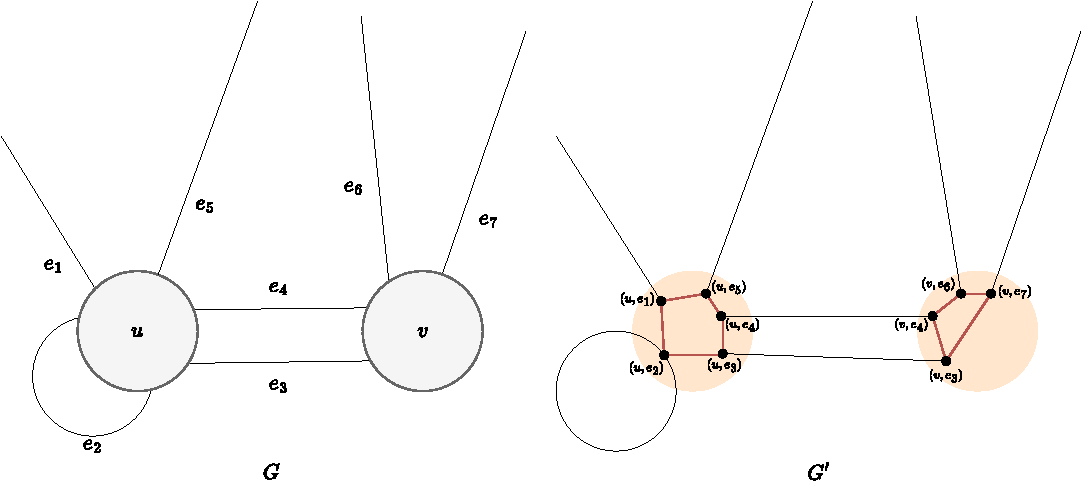
\includegraphics[width=\textwidth]{images/degree_reduction.pdf}
  \caption{次数削減変換の例. 橙色の内部の頂点集合がクラウドであり, クラウド内の辺は\cref{thm:construction-of-expander-graph}によって構成されるが, ここでは図の簡単のため$X_d$を長さ$d$の閉路としている. $G'$における黒い辺の制約は対応する元のグラフの辺と同一の制約とし, クラウド内の赤辺の制約は等式制約とする.}
  \label{fig:degree-reduction}
\end{figure}

元のグラフの各頂点$u\in V$に対し, 
\[[u]=\qty{ (u,e) \in \{u\}\times E \colon e=\{u,v\} \text{ for some } v\in V }\]
を(この証明のローカルな用語として)\emph{$u$-クラウド}と呼ぶことにする.
新しい頂点集合$V'$は$V'=\bigcup_{u\in V} [u]$である.
すなわち, $u$をそれに接続する辺の本数(自己ループは1個分としてカウント)だけコピーして得られる集合が$[u]$である.

次に辺集合$E'$を以下のように構成する.
まず, $(X_n)_{n\in\Nat}$を\cref{thm:construction-of-expander-graph}によって構成される$n$頂点$d_0$-正則$\lambda$-エクスパンダーの族とする.
元のグラフの各頂点$u\in V$に対し, $d=\abs{[u]}$としたとき, 頂点集合$[u]$上で$X_d$と同型なグラフを構成し, それを$([u],E_u)$とする.
このとき, 各$u$-クラウド内部の辺集合$E_{\mathrm{inner}}$は
\begin{align*}
  E_{\mathrm{inner}} = \bigcup_{u\in V} E_u
\end{align*}
とする.
次に異なるクラウド間を繋ぐ辺集合$E_{\mathrm{outer}}$を
\begin{align*}
  E_{\mathrm{outer}} = \qty{\qty{ (u,e), (v,e) } \colon e\notin [u]\cap[v]}
\end{align*}
とする.
このとき, グラフ$G'$の辺集合$E'$は
\begin{align*}
  E' = E_{\mathrm{inner}} \cup E_{\mathrm{outer}}
\end{align*}
となる.

次に各辺$e'\in E'$の制約$c'_{e'}$を以下のように定める:
\begin{itemize}
\item 辺$e'\in E_{\mathrm{outer}}$がクラウド間をつなぐ辺ならば, その制約は対応する元の辺$e$の制約と同じとする.
すなわち, $e'=\qty{ (u,e), (v,e) }$ならば, $c'_{e'}=c_e$である.
\item 辺$e'\in E_{\mathrm{inner}}$がクラウド内部の辺ならば, その制約を$c'_{e'}=\{(\sigma,\sigma)\colon \sigma\in\Sigma\}$, すなわち等式制約とする.
\end{itemize}

このようにして得られる制約グラフ$G'=\ip{(V',E'),\Sigma,\calC'}$が補題の主張を全て満たすことを確認する.
まず, $G'$は$(d_0+1)$-正則である.
実際, $G'$の各頂点$(u,e)\in V'$に接続する辺は, クラウド内の辺が$d_0$本, クラウド間の辺が$1$本である.
また, $G$から$G'$を構成する際に新たに追加する辺は$E_{\mathrm{inner}}$のみであり, これは高々$\sum_{u\in V}\frac{d_0\deg_G(u)}{2} \le d_0\abs{E}$本である (ここで\cref{eq:hand_shake_multigraph}を用いた).
従って
\begin{align}
  \abs{E'} = \abs{E_{\mathrm{inner}}} + \abs{E_{\mathrm{outer}}} \le \qty(d_0+1)\abs{E} \label{eq:bound_of_E'}
\end{align}
を満たす.
また, $V'$の要素数は次数の総和に等しいため, $\abs{V'}\le 2\abs{E}$を満たす.
次に, $\UNSAT(G)=0$ならば$\UNSAT(G')=0$である.
実際, 元の制約グラフの全ての制約を満たす割り当て$a\colon V\to\Sigma$に対し, $G'$の割り当て$a'\colon V'\to\Sigma$を
\begin{align*}
  a'(u,e) = a(u)
\end{align*}
と定めると, $a'$は$G'$の制約を満たす (同一クラウド内の頂点には全て同じ値が割り当てられるため, クラウド内の辺の制約は全て満たされ, クラウド間の辺に対応する制約は$a$の取り方により全て満たされることがわかる).

最後の主張, すなわち$\UNSAT(G') \ge c'\cdot \UNSAT(G)$となる定数$c'>0$が存在すること示す.
定数$c'>0$を
\begin{align}
  c' = \min\qty{\frac{(1-\lambda_0)d_0}{8(d_0+1)}, \frac{1}{2(d_0+1)}} \label{eq:c_of_degree_reduction}
\end{align}
と定める.
$\UNSAT(a';G')=\UNSAT(G')$を満たす割り当て$a'\colon V'\to\Sigma$を任意に取る.
この割り当て$a'$に対し, 元のグラフ$G$の割り当て$a\colon V\to\Sigma$を
\begin{align*}
  a(u) = \Maj((a'(u,e))_{(u,e) \in [u]})
\end{align*}
と定める. ここで$\Maj(\cdot)$は多数決関数であり,
タイは任意に選ぶとする.
例えば$\Maj(1,2,2)=2$, $\Maj(1,2,3,3)=3$, $\Maj(1,2,2,3,3)=2$である ($\Maj(1,2,2,3,3)=3$としても良いが, ここでは便宜上小さい方の数字を採用している).

以降, 割り当て$a'\colon V'\to\Sigma$に対し, 頂点$(u,e)\in V'$への割り当て$a'(u,e)$を頂点$(u,e)$の\emph{意見}と呼ぶこととする.
同様に, 割り当て$a\colon V\to\Sigma$に対し, 頂点$u\in V$への割り当て$a(u)$を頂点$u$の意見と呼ぶこととする.
直感的には頂点$u$の意見は対応する$u$-クラウド内の頂点の意見の多数決である.


辺集合$F\subseteq E$を割り当て$a$によって充足されない辺の集合, すなわち
\begin{align*}
  F = \qty{ e=\{u,v\}\in E \colon (a(u),a(v)) \not\in c_e}
\end{align*}
と定義する.
ここで$\calC = (c_e)_{e\in E}$は元の制約グラフ$G$の制約である.
同様に, $F'\subseteq E'$を割り当て$a'$によって充足されない辺の集合とする.
このとき$\UNSAT(a;G) = \frac{|F|}{|E|}$および$\UNSAT((a';G') = \frac{|F'|}{|E'|}$である.
頂点部分集合$S\subseteq V'$を$a$の多数決で選ばれなかった意見を持つ頂点の集合, すなわち
\begin{align*}
  S = \qty{ (u,e) \in V' \colon a(u) \ne a'(u,e)}
\end{align*}
と定義し, 各$v\in V$に対し$S^v = S\cap [v]$とし, 各$\sigma\in \Sigma$に対し$S^v_\sigma = \qty{ (u,e)\in S^v \colon a'(u,e)=\sigma }$とする (\cref{fig:majority-degree-reduction}).
なお, $\sigma\in\Sigma$が多数決の意見 (すなわち$\sigma=a(v)$)のとき, $S^v_\sigma=\emptyset$とする.

\begin{figure}[ht]
  \centering
  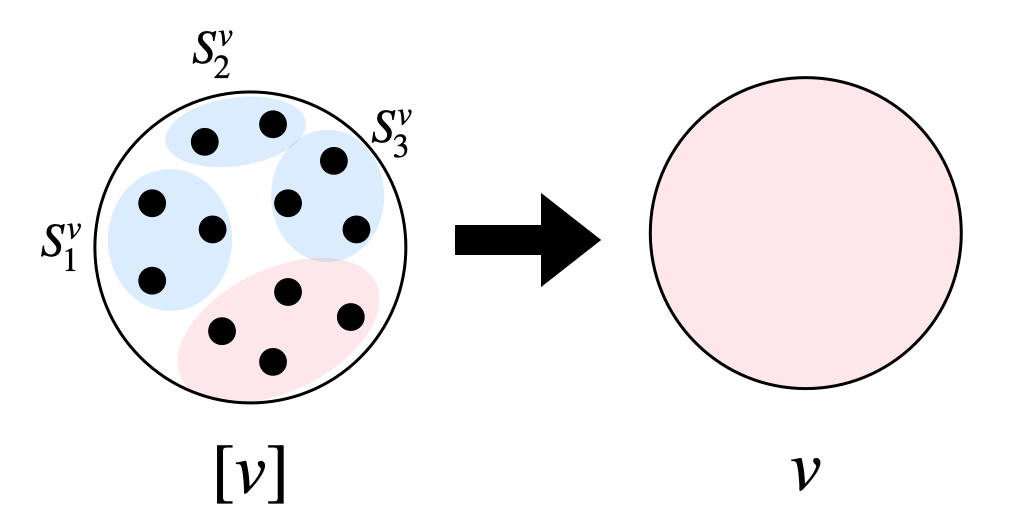
\includegraphics[width=\textwidth]{images/majority_degree_reduction.png}
  \caption{多数決によって選ばれなかった$v$-クラウド内の頂点の集合を$S_v\subseteq [v]$とする. \label{fig:majority-degree-reduction}}
\end{figure}

以下の二つのケースを考える:

\paragraph*{ケース1. $\abs{S} \ge \frac{\UNSAT(a;G)}{2}\abs{E}$の場合.}

各頂点$v\in V$と多数決によって選ばれなかった意見$\sigma\in\Sigma \setminus \{a(v)\}$に対し$\abs{S^v_\sigma} \le \frac{\abs{[v]}}{2}$である
(そうでなければ意見$\sigma$が多数決によって選ばれなかったことに矛盾する).
ここで$v$-クラウド内部のグラフは$d_0$-正則$\lambda_0$-エクスパンダーであるため, その頂点部分集合$S^v_\sigma\subseteq[v]$に対するエクスパンダー混交補題(\cref{lem:expander-mixing-lemma})より,
\begin{align*}
  W(S^v_\sigma, [v]\setminus S^v_\sigma) \ge (1-\lambda_0)\cdot \frac{d_0\abs{S^v_\sigma}}{2}
\end{align*}
となる. ここで$W(S,T)$は$v$-クラウド内部のグラフ$([v],E_v)$の辺であって$S$と$T$の間をまたがる辺の本数である.
ここで$S^v_\sigma$と$[v]\setminus S^v_\sigma$をまたがる全ての辺の両端点の意見は異なるため, $a'$はこれらの辺を充足しない. よってこれらの辺は全て$F'$に含まれる.
従って
\begin{align*}
  \abs{F'} &\ge \frac{1}{2}\sum_{v,\sigma} W(S^v_\sigma, [v]\setminus S^v_\sigma) \\
  &\ge \frac{(1-\lambda_0)d_0}{4}\sum_{v,\sigma} \abs{S^v_\sigma} \\
  &= \frac{(1-\lambda_0)d_0}{4}\abs{S} \\
  &\ge \frac{(1-\lambda_0)d_0}{8}\UNSAT(a;G)\cdot \abs{E}  & & \because \text{ケース1の仮定} \\
  &\ge \frac{(1-\lambda_0)d_0}{8(d_0+1)}\UNSAT(a;G)\cdot \abs{E'}. & & \because\text{\cref{eq:bound_of_E'}}
\end{align*}
特にこれから$\UNSAT(a';G') = \frac{\abs{F'}}{\abs{E'}}\ge \frac{(1-\lambda_0)d_0}{8(d_0+1)}\cdot\UNSAT(a;G)$が成り立つ.

\paragraph*{ケース2. $\abs{S} < \frac{\UNSAT(a;G)}{2}\abs{E}$の場合.}
任意の辺$e = \{u,v\} \in F$に対して, それに対応する$G'$の辺$e' = \{(u,e),(v,e)\}$を考える.
\begin{itemize}
\item もしも$a(u)=a'(u,e)$かつ$a(v)=a'(v,e)$が成り立つならば, $e'$と$e$は同じ制約を持ち, $e\in F$であることから$e'\in F'$である.
\item そうでない, すなわち$a(u)\ne a'(u,e)$または$a(v)\ne a'(v,e)$が成り立つならば, $(u,e)$と$(v,e)$のうち少なくとも一方はその意見が多数決として選ばれない, すなわち$(u,e)\in S$または$(v,e)\in S$が成り立つ.
\end{itemize}
以上より$\abs{F} \le \abs{F'} + \abs{S}$が成り立つので
\begin{align*}
  \abs{F'} &\ge \abs{F} - \abs{S} \\
  &\ge \abs{E}\UNSAT(a;G) - \frac{\UNSAT(a;G)}{2}\abs{E} & & \because \text{ケース2の仮定}\\
  &= \frac{\UNSAT(a;G)}{2}\abs{E} \\
  &\ge \frac{\UNSAT(a;G)}{2(d_0+1)}\abs{E'} & & \because\text{\cref{eq:bound_of_E'}}
\end{align*}
となり, これから
\begin{align*}
  \UNSAT(a';G') = \frac{\abs{F'}}{\abs{E'}} \ge \frac{1}{2(d_0+1)}\cdot \UNSAT(a;G)
\end{align*}
が成り立つ.

ケース1,2より, \cref{eq:c_of_degree_reduction}で定まる定数$c'>0$に対して$\UNSAT(a';G') \ge c'\cdot \UNSAT(a;G) \ge c'\cdot \UNSAT(G)$が成り立つ.
\end{proof}

\subsection{エクスパンダー化}

次に, 与えられた正則な制約グラフをエクスパンダーグラフに変換する補題を示す.

\begin{lemma}{エクスパンダー化補題}{expanderization}
ある定数$\lambda<1,d,d_0\in\Nat$および次を満たす多項式時間アルゴリズム$A$が存在する:
アルゴリズム$A$は入力として$d$-正則な制約グラフ$G = \ip{ (V,E), \Sigma, \calC }$
を受け取り, $(d+d_0+1)$-正則で全頂点が自己ループを持ち, さらに$\lambda$-エクスパンダーである制約グラフ $G' = \ip{ (V, E'), \Sigma, \calC' }$ を出力する.
さらに, この制約グラフ$G'$は$\UNSAT(G') = \frac{d}{d+d_0+1}\UNSAT(G)$を満たす.
\end{lemma}

\begin{proof}
入力として与えられた制約グラフを$G=\ip{(V,E),\Sigma,\calC}$とする.
変換は以下のようにして行われる:
\begin{enumerate}
\item まず, \cref{thm:construction-of-expander-graph}を用いて頂点集合$V$上$d_0$-正則$\lambda_0$-エクスパンダーグラフを構成し, その辺集合を$E$に追加する (この際多重辺も許す).
\item 次に, 各頂点に自己ループを付与する.
\item ステップ1,2で追加した辺$e$に対応する制約$c'_e$を自明な制約$c'_e=\Sigma^2$とする.
\end{enumerate}
このようにして得られる制約グラフを$G'=\ip{(V',E'),\Sigma,\calC'}$とする.
元の制約グラフ$G$が$d$-正則であることから, $G'$は$(d+d_0+1)$-正則である (自己ループの次数への寄与は$1$であることに注意).
また, ステップ2より$G'$は全頂点が自己ループを持つ.

次に$\UNSAT(G')=\frac{d}{d+d_0+1}\UNSAT(G)$を示す.
任意の割り当て$a\colon V \to \Sigma$に対し, 
ステップ1,2で追加した辺に対応する制約は常に充足されるため, 両者が充足\emph{しない}制約の個数は一致する.
すなわち$\abs{E}\UNSAT(a;G) = \abs{E'}\UNSAT(a;G')$が成り立つので
\begin{align*}
  \UNSAT(G') = \min_{a}\UNSAT(a;G') = \frac{\abs{E}}{\abs{E'}}\min_a \UNSAT(a;G) = \frac{d}{d+d_0+1}\UNSAT(G)
\end{align*}
が成り立つ.

最後に$G'$が$\lambda:=\frac{d}{d+d_0+1}+\frac{\lambda_0(d_0+1)}{d+d_0+1}$に対し$\lambda$-エクスパンダーであることを示す.
元のグラフ$G$の遷移確率行列を$P\in[0,1]^{V\times V}$とし,
ステップ1,2で追加した辺からなるグラフを$G_0$とし, その遷移確率行列を$P_0\in[0,1]^{V\times V}$とする.
また, 最終的に得られるグラフ$G'$の遷移確率行列を$P'\in[0,1]^{V\times V}$とする.
元のグラフ$G$は$d$-正則, 追加したグラフ$G_0$は$(d_0+1)$-正則であるため
\begin{align*}
  P' = \frac{d}{d+d_0+1}P + \frac{d_0+1}{d+d_0+1}P_0
\end{align*}
となる.
さらに$P_0$は$\lambda_0$-エクスパンダーであるため, 全成分$1$のベクトル$\allone$と直交する任意のベクトル$x\in \Real^V$に対し
\begin{align*}
  x^\top P' x &= \frac{d}{d+d_0+1}x^\top P x + \frac{d_0+1}{d+d_0+1}x^\top P_0 x \\
  &\ge \frac{d}{d+d_0+1}\norm{x}^2 + \frac{d_0+1}{d+d_0+1}\lambda_0\norm{x}^2 & & \because\text{$P_0$のエクスパンダー性}\\
  &\le \qty( \frac{d}{d+d_0+1} + \frac{\lambda_0(d_0+1)}{d+d_0+1} )\norm{x}^2
\end{align*}
より, $\lambda(P')\le \frac{d}{d+d_0+1} + \frac{\lambda_0(d_0+1)}{d+d_0+1}$が成り立つ.
\end{proof}

これにより\cref{lem:constant-degree-expanderization}を示す準備が整った.
\begin{proof}[\cref{lem:constant-degree-expanderization}の証明]

与えられた制約グラフ$G$に対し, まず$G$を入力として\cref{lem:degree-reduction}のアルゴリズムを実行し, その出力を$G_1$とする.
この制約グラフ$G_1$は\cref{lem:degree-reduction}の主張より, $d$-正則である.
次に, $G_1$を入力として\cref{lem:expanderization}のアルゴリズムを実行し, その出力を最終的な出力$G$とする.
この制約グラフ$G'$は\cref{lem:expanderization}の主張より, 全頂点が自己ループを持ち, $(d+d_0+1)$-正則かつ$\lambda$-エクスパンダーである.
また, この一連の変換によって$\size(G')$は$\size(G)$の定数倍にしかならない.

最後に$\UNSAT$の値を考える.
元の制約グラフ$G$が$\UNSAT(G)=0$ならば, \cref{lem:degree-reduction,lem:expanderization}より
$\UNSAT(G') = \frac{d}{d+d_0+1}\UNSAT(G_1) = 0$を得る.
一方で
\begin{align*}
  \UNSAT(G') = \frac{d}{d+d_0+1}\UNSAT(G_1) \ge \frac{d}{d+d_0+1}\cdot c'\cdot\UNSAT(G).
\end{align*}
すなわち$\beta = \frac{d}{d+d_0+1}\cdot c'$に対して主張が成り立つことが示された.
\end{proof}

\section{制約グラフのべき乗}

\cref{lem:constant-degree-expanderization}により, 任意の制約グラフを定数次数エクスパンダーに変換することができる.
この節では, そのような制約グラフに対し, 以下で定義する\emph{べき乗}という操作を考えることで, その$\UNSAT$の値を増幅させることができることを示す.

\begin{definition}{制約グラフの冪乗}{power-of-constraint-graph}
  パラメータ$\ell\in\Nat$および全頂点が自己ループを持つ$d$-正則な制約グラフ$G=\ip{(V,E),\Sigma,\calC}$に対し, べき乗$G^\ell = \ip{(V,\boldE),\Sigma^{d^{\ell}},\calC^\ell}$を, 以下のようにして定義する:
  \begin{itemize}
    \item 頂点集合は同じ$V$とする. なお, $V$の元は$v_1<\dots < v_n$のように順序づけられているとする.
    \item グラフ$(V,\boldE)$をべき乗(\cref{def:power-of-graph})によって得られるグラフ$(V,E)^\ell$とする. すなわち, 各二頂点$u,v\in V$に対し, 長さ$\ell$の$uv$-路の個数と同じだけ$uv$間に多重辺を用意する ($uv$-路と$vu$路の個数は一致するため, 無向グラフとして定義できる). このようにして得られる辺の多重集合を$\boldE$とし, その元を$\bolde = \{u,v\} \in \boldE$とする.
    \item アルファベット集合は$\Sigma^{d^{\ell}}$とする. ここで, 頂点$u$に$\vec{\sigma}=(\sigma_1,\dots,\sigma_{d^{\ell}}) \in \Sigma^{d^{\ell}}$が割り当てられたとき, 次の意味を持つ: 元の$d$-正則グラフ$G$上で頂点$u$から距離$\ell$以内の頂点の集合を$\Gamma(u)$とし\footnote{頂点$v$が頂点$u$から距離$i$以内であるというのは, 頂点$u$から開始し頂点$v$に至る長さ$i$以下の路が存在することをいう.}, その元を頂点番号の大小順で並べて$\Gamma(u)=\qty{ v_1,\dots,v_\ell}$ とする (ここで$G$の$d$-正則性より$\ell \le d^{\ell}$である). このとき, $\vec{\sigma}$は各$v\in\Gamma(u)$に$\vec{\sigma}_u\in \Sigma$を割り当てる写像とみなし, $\vec{\sigma}_v$を\emph{$u$の$v$に対する意見}と呼ぶ.
    なお, $\ell < d^{\ell}$の場合は相異なる二つの$\vec{\sigma},\vec{\sigma}'\in\Sigma^{d^{\ell}}$が同一の写像としてみなされることもある (これらは制約を充足するか否かにおいては区別されない).
    \item 辺$\bolde = \{u,v\} \in \boldE$ に対応する制約$\boldc_{\bolde}\in \calC^\ell$は次の二つを満たす割り当て$(\vec{\sigma},\vec{\sigma}')\in \Sigma^{d^{\ell}} \times \Sigma^{d^{\ell}}$によって満たされる:
    元のグラフ$G$の全ての辺$e=\{s,t\}\in E$ (ただし$s<t$)に対し,
      \begin{itemize}
        \item $s\in \Gamma(u), t\in\Gamma(v)$ならば$(\vec{\sigma}(s), \vec{\sigma}'(t))\in c_e$が成り立つ.
        \item $s\in\Gamma(v), t\in\Gamma(u)$ならば$(\vec{\sigma}'(s), \vec{\sigma}(t))\in c_e$が成り立つ.
      \end{itemize}
  \end{itemize}
\end{definition}

\begin{figure}[ht]
  \centering
  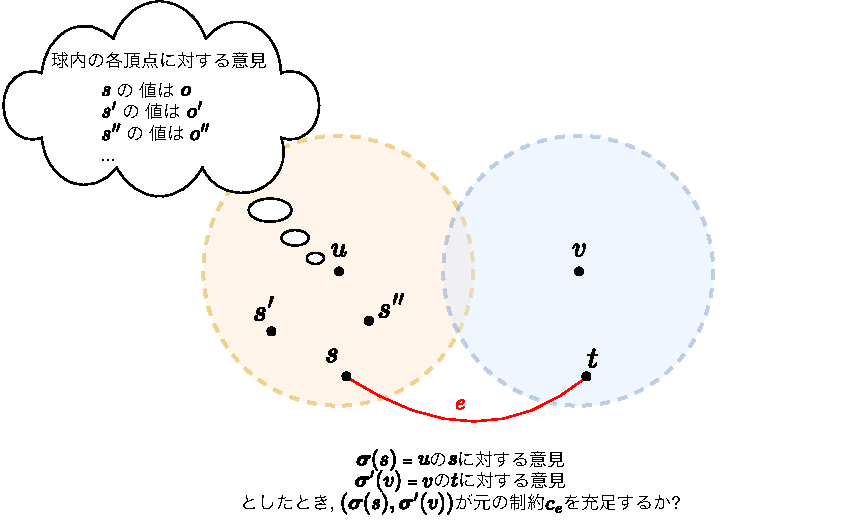
\includegraphics[width=\textwidth]{images/gap_amplification.pdf}
  \caption{制約グラフ$G$のべき乗$G^\ell$の図例. 頂点$u,v$にそれぞれ$\vec{\sigma},\vec{\sigma}'\in\Sigma^{d^{\ell}}$が割り当てられているとき, それぞれ関数$\vec{\sigma}\colon \Gamma(u)\to\Sigma$と$\vec{\sigma}'\colon \Gamma(v)\to\Sigma$とみなす. なお, 元のグラフ$G$が自己ループを持つことから, 距離$\ell$以内の全ての頂点に対して意見が定義される.\label{fig:gap-amplification}}
\end{figure}

最後に, $G^\ell$における割り当て$a'\colon V\to\Sigma^{d^{\ell}}$に対し, $u$の$w$に対する意見を$a'(u)_w$と表すことにする.

パラメータ$\ell$は制約グラフのサイズ$\size(G)$には依存しない定数であることを常に想定する.
べき乗をで得られた制約グラフは元の制約グラフに対して$\UNSAT$の値が増幅している.

\begin{lemma}{べき乗の性質}{property-of-power}
  ある定数$\beta=\beta(\lambda,d,\abs{\Sigma})$が存在して以下が成り立つ:
  十分大きいパラメータ$\ell=\ell(d,\abs{\Sigma},\lambda) \le \abs{E}$および全頂点が自己ループを持つ$d$-正則な制約グラフ$G=\ip{(V,E),\Sigma,\calC}$に対し, べき乗$G^\ell = \ip{(V,\boldE),\Sigma^{\ell},\calC^\ell}$を, \cref{def:power-of-constraint-graph}で定義する.
  このとき
  \begin{itemize}
    \item $\size(G^\ell) \le \size(G)\cdot d^\ell$である.
    \item $\UNSAT(G)=0$ならば$\UNSAT(G^\ell)=0$である.
    \item $\UNSAT(G^\ell) \ge \beta\sqrt{\ell}\cdot \min\qty{ \UNSAT(G), \frac{1}{\ell} }$である.
  \end{itemize}
\end{lemma}

\begin{remark}{「定数」の意味}{mean-of-constants}
  主張や証明の中でしばし「定数」という言葉を多用するが, ここでは$d,\lambda,\abs{\Sigma}$をユニバーサルな定数で固定し, これらの値に応じて定まる値$\beta,\ell$なども定数と呼ぶ.
  ただし, 定数はグラフの頂点数や辺数には依存しない.
\end{remark}

\begin{proof}

定義より$\abs{\boldE} \le \abs{V}d^{\ell}$であるから, $\size(G^\ell) \le \size(G)\cdot d^\ell$である.

また, $\UNSAT(G)=0$ならば, 全制約を満たす割り当て$a\colon V \to \Sigma$に対し, $a'(u)$に
\begin{align*}
  \vec{\sigma}(u)\colon w \mapsto a(w)
\end{align*}
で定まる関数$\vec{\sigma}\colon \Gamma(w)\to\Sigma$とみなせる値$\vec{\sigma}\in\Sigma^{d^\ell}$を割り当てる (候補が複数存在する場合はどれでもよい).
このようにして定まる$a'\colon V\to\Sigma^{\ell}$を考えると, これは全ての制約を満たす割り当てであるため, $\UNSAT(G^\ell)=0$である.

最後に$\UNSAT(G^\ell)$の下界を証明する.
簡単のため$\ell$は偶数であるとする (奇数の場合は$\ell/2$を$\floor{\ell/2}$に置き換えれば同じ証明が成立する).
頂点$u\in V$に対し, $V$値をとる確率変数$\RW_j(u)$を, グラフ$G$上で頂点$u$から開始する長さ$j$のランダムウォークの最終到達頂点とする (長さとは辿った辺の本数のことである).
べき乗の制約グラフ$G^\ell$における割り当て$a'\colon V \to \Sigma^{\ell}$に対し, 元の制約グラフに対する任意の割り当て$a\colon V\to\Sigma$を
\begin{align}
  a(u) = \argmax_{\tau \in \Sigma} \qty{ \Pr\qty[ a'(\RW_{\ell/2}(u))_u = \tau ] }. \label{eq:argmax-of-RW}
\end{align}
によって定める.
常に$\RW_{\ell/2}(u)\in \Gamma(u)$であるから$a'(\RW(u))_u$は必ず存在する.
すなわち, $u$から開始したランダムウォークが最も「拾いやすい」意見を$a(u)$としている.
このようにして定めた割り当て$a\colon V \to \Sigma$は, 適当な定数$\beta=\beta(\lambda,d,\abs{\Sigma})>0$に対して
\begin{align}
  \UNSAT(a';G^\ell) \ge \beta\sqrt{\ell}\cdot \min\qty{ \UNSAT(a;G), \frac{1}{\ell} }. \label{eq:lower-bound-of-UNSAT}
\end{align}
を満たすことを後で示す. $\UNSAT(a';G^\ell)=\UNSAT(G^\ell)$を満たす$a'$に対して\cref{eq:lower-bound-of-UNSAT}を適用し, さらに$\UNSAT(a;G)\le \UNSAT(G)$を代入すると$\UNSAT(G^\ell)$の所望の下界が得られて証明は完了する.

\paragraph*{\cref{eq:lower-bound-of-UNSAT}の証明.}

割り当て$a'\colon V\to \Sigma^{d^{\ell}}$を固定し, $a$を\cref{eq:argmax-of-RW}によって定める.
辺部分集合$F_0\subseteq E$を, $a$によって充足されない辺の集合とし,
さらにその部分集合$F\subseteq F_0$を, 
\begin{itemize}
\item $\abs{F_0} \le \frac{\abs{E}}{\ell}$ならば$F_0=F$,
\item そうでない場合は$\abs{F} = \floor*{\frac{\abs{E}}{\ell}}$となるように$F$を任意に固定する.
\end{itemize}
このとき, 任意の$x\ge 1$に対し$\floor{x}\ge x/2$であることから, $\frac{\abs{E}}{\ell}\ge 1$の仮定を用いて
\begin{align}
  \abs{F} &\ge \min\qty{ \abs{F_0}, \floor*{\frac{\abs{E}}{\ell}} } \nonumber \\
  &\ge \frac{1}{2}\min\qty{ \abs{F_0}, \frac{\abs{E}}{\ell} } \nonumber \\
  &\ge \frac{\abs{E}}{2}\min\qty{ \UNSAT(a;G), \frac{1}{\ell} } \label{eq:abs-F}
\end{align}
を得る (なお, $\abs{E}\ge \ell$の仮定を用いるのはここのみである).

べき乗グラフの辺$\bolde \in \boldE$は$G$上の長さ$\ell$の路に対応する.
従って$\bolde = (u_0,\dots,u_\ell)$ (ただし全ての$i\in[\ell]$に対し$\qty{u_{i-1},u_{i}}\in E$)と表し, 元のグラフの辺と区別するため$e\in E$を$G$辺, $\bolde\in\boldE$を$G^\ell$辺と呼ぶことにする.

$G^\ell$辺$\bolde=(u_0,\dots,u_\ell)$の$i$番目の辺$e_i:=\qty{u_{i-1},u_i}$は
\begin{itemize}
  \item $e_i \in F$
  \item $a'(u_{0})_{u_{i-1}} = a(u_{i-1})$ かつ $a'(u_\ell)_{u_i} = a(u_i)$
\end{itemize}
をどちらも満たすとき, \emph{悪い}ということにする.
一様ランダムに$\bolde$を選んだとき, $B_i\in\binset$を辺$e_i$が悪いならば$B_i=1$, そうでないならば$B_i=0$とする (これらは確率変数である).
さらに
\begin{align*}
  I = \qty[\frac{\ell}{2} - \sqrt{\ell}, \frac{\ell}{2} + \sqrt{\ell}] \cap \mathbb{Z}
\end{align*}
に対し, $B=\sum_{i\in I}B_i$とする.
もしも$B>0$ならば, 辺$\bolde$の制約$c'_{\bolde}$は$a'$によって充足されない.
従って, $\UNSAT(a';G^\ell) \ge \Pr_{\bolde\sim \boldE}[B\ge 1]$である.

Paley-Zygmundの不等式(\cref{lem:paley-zigmund-inequality})より, $\E[B]$および$\E[B^2]$を評価することで$\Pr[B\ge 1]$の下界を得ることができる.
これらは以下のように評価できる. 

\begin{claim}{$B$の期待値}{expectation-of-B}
  ある十分小さな定数$C=C(d,\lambda,\abs{\Sigma})>0$が存在して, $B$の期待値は
  \begin{align*}
    \E[B] \ge C\sqrt{\ell} \cdot \frac{\abs{F}}{\abs{E}}.
  \end{align*}
\end{claim}

\begin{claim}{$B^2$の期待値}{expectation-of-B-squared}
  ある十分大きな定数$C'=C'(d,\lambda,\abs{\Sigma})>0$が存在して, $B^2$の期待値は
  \begin{align*}
    \E[B^2] \le C'\sqrt{\ell} \cdot \frac{\abs{F}}{\abs{E}}.
  \end{align*}
\end{claim}

これらの主張の証明は後で与える.
ここでは, これらを用いて\cref{eq:lower-bound-of-UNSAT}を示す.
実際, \cref{lem:paley-zigmund-inequality,claim:expectation-of-B,claim:expectation-of-B-squared}より, 定数$\beta=\frac{C^2}{2C'}>0$に対して
\begin{align*}
  \UNSAT(a';G^\ell) &\ge \Pr[B\ge 1] \\
  &\ge \frac{\E[B]^2}{\E[B^2]} \\
  &\ge \frac{C^2}{C'} \sqrt{\ell} \cdot \frac{\abs{F}}{\abs{E}} \\
  & \ge \beta \sqrt{\ell} \cdot \min\qty{ \UNSAT(a;G), \frac{1}{\ell} } & & \because \text{\cref{eq:abs-F}}
\end{align*}
となり主張を得る.

\end{proof}

最後に残された二つの主張の証明を与える. なお, 制約グラフのエクスパンダー性を用いるのは\cref{claim:expectation-of-B-squared}の証明のみである.
\begin{proof}[\cref{claim:expectation-of-B}の証明]
  各$i\in I$に対して$\E[B_i]=\Pr_{\bolde\sim \boldE}[e_i\text{ が悪い}]$を下から抑えればよい.
  一様ランダムな$\bolde=(u_0,\dots,u_\ell)\sim\boldE$は$G$上の長さ$\ell$のランダムウォークであるから, 各$i\in I$に対して$\bolde$は以下のプロセスによって生成される:
  \begin{enumerate}
    \item 辺$\{u_{i-1},u_i\}\sim E$を一様ランダムに選ぶ.
    \item 頂点$u_{i-1}$から開始して長さ$i-1$のランダムウォークを行い, 辿った頂点を順番に$u_{i-1},u_{i-2},\dots,u_0$とする.
    \item 同様に, 頂点$u_i$から開始して長さ$\ell-i$のランダムウォークを行い, 辿った頂点を順番に$u_i,u_{i+1},\dots,u_\ell$とする.
    \item 頂点列$(u_0,\dots,u_\ell)$に対応する$\bolde \in \boldE$を出力する.
  \end{enumerate}

  \begin{figure}[ht]
    \centering
    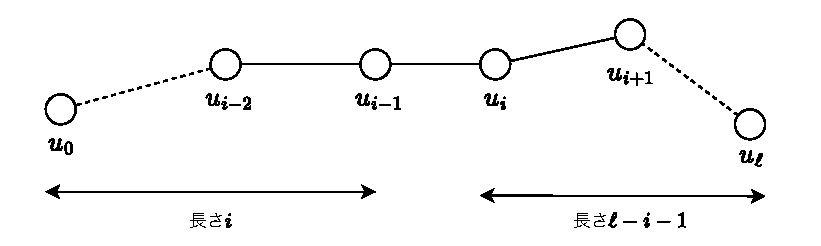
\includegraphics[width=0.9\textwidth]{images/randomwalk_process.pdf}
    \caption{ランダムウォークの図例. 頂点$u_0$から開始して長さ$i-1$のランダムウォークを行い, 辿った頂点を順番に$u_{i-1},u_{i-2},\dots,u_0$とする. 同様に, 頂点$u_i$から開始して長さ$\ell-i$のランダムウォークを行い, 辿った頂点を順番に$u_i,u_{i+1},\dots,u_\ell$とする. この二つのランダムウォークを組み合わせて, 長さ$\ell$のランダムウォークを生成する. \label{fig:random-walk}}
  \end{figure}

  このプロセスに基づいて, $\Pr[B_i=1]$を評価する.
  まず, ステップ1で選ばれた辺が$\qty{u_{i-1},u_i}\in F$である確率は$\frac{\abs{F}}{\abs{E}}$である.
  次にステップ1で選ばれた辺$\qty{u_{i-1},u_i}\in F$で条件つけたとき, ステップ2と3は独立なランダムネスに基づく試行であるため, それぞれの両端点$u_0,u_\ell$は独立な確率変数である.
  従って
  \begin{align}
    \Pr[B_i=1] &= \E_{\text{step 1-3}}\qty[\{u_{i-1},u_i\}\in F \text{ and }a'(u_0)_{u_{i-1}} = a(u_{i-1})\text{ and }a'(u_\ell)_{u_i} = a(u_i)] \nonumber \\
     &= \frac{\abs{F}}{\abs{E}} \cdot \E_{\{u_{i-1},u_i\}\sim F}\qty[ \underbrace{\Pr_{\text{step 2}}[a'(u_0)_{u_{i-1}} = a(u_{i-1})]}_{=:p_0} \cdot \underbrace{\Pr_{\text{step 3}}[a'(u_\ell)_{u_i} = a(u_i)]}_{=:p_\ell}] \label{eq:Pr-B_i}
  \end{align}
  を得る. 二つ目の等式では, $\{u_{i-1},u_i\}\in F$で条件つけて$\{u_{i-1},u_i\}\sim E$をランダムに選ぶというのは, $F$内の辺を一様ランダムに選ぶことに他ならないことに留意する.

  次に, $p_0$と$p_\ell$を評価する.
  頂点$u_{i-1}$を任意に固定して$p_0$を考える ($p_\ell$も同様に示せる).
  頂点$u\in V$および非負整数$m\ge 0$に対し, 確率変数$X_{u,m}\in\Sigma$を, ($a'$における)$\RW_m(u)$の$u$に対する意見, すなわち$X_{u,m} = a'(\RW_m(u))_u$とする.
  \cref{eq:argmax-of-RW}より, $m=\ell/2$のとき, 
  \begin{align}
  \Pr[X_{u_{i-1},\ell/2} = a(u_{i-1})] \ge \frac{1}{\abs{\Sigma}} \label{eq:center_opinion}
  \end{align}
  である.
  ステップ2で選ばれた端点$u_0$は$u_0=\RW_i(u_{i-1})$であるから, $X_{u_{i-1},i}=a'\qty( \RW_i(u_{i-1}) )_{u_{i-1}} = a'\qty(u_0)_{u_{i-1}}$である.
  従って, 
  \begin{align}
    p_0 = \Pr[X_{u_{i-1},i} = a(u_{i-1})] \label{eq:p_0}
  \end{align}
  である. 任意に頂点$u\in V$と$i\in I$を固定して$X_{u,\ell/2}$と$X_{u,i}$の分布を比較する.
  $i\in I$なので, $\abs{i-\ell/2} \le \sqrt{\ell}$である.

  元のグラフ$G$の各頂点に対し, その頂点が持つ自己ループの一つを赤く塗る
  (仮定より元のグラフ$(V,E)$は$d$-正則かつ各頂点が自己ループを少なくとも一つ持つ).
  頂点$u$から開始する長さ$\ell/2$のランダムウォークを考え,
  確率変数$Y_{\ell/2}$を, このランダムウォークが辿った赤\emph{以外}の辺の個数とする ($Y_i$も同様に定義する).
  各頂点がちょうど一つの赤い自己ループを持つため,
  確率変数$Y_{\ell/2}$の分布は始点$u$に依存せず二項分布$\Bin(\ell/2,1-1/d)$である (同様に$Y_i$の分布は$\Bin(i,1-1/d)$である).
  また, $\RW'_k(u)$を, 頂点$u$から開始する赤い辺を選ばない長さ$k$のランダムウォークの最終到達頂点とする (すなわち, $G$の各頂点から赤い辺を除いて得られるグラフ上の長さ$k$のランダムウォークである).
  従って, 任意の頂点部分集合$A\subseteq V$に対し
  \begin{align}
    \Pr\qty[\RW_{i}(u)\in A] &= \sum_{k=0}^{i} \Pr\qty[\RW_{i}(u) \in A \condition Y_{i}=k] \cdot \Pr\qty[Y_{i}=k] \nonumber \\
    &= \sum_{k=0}^{i} \Pr\qty[\RW'_k(u) \in A] \cdot \Pr\qty[Y_{i}=k] \label{eq:RW_i_distribution}
  \end{align}
  が成り立つ.
  ここで, 以下の主張を後で示す:
  \begin{claim}{}{two-constants}
  十分大きな定数$C_1=C_1(d,\abs{\Sigma})>0$と十分小さな定数$C_2=C_2(d,\abs{\Sigma})>0$が存在して以下が成り立つ:
  $K:= \qty{ k\in \mathbb{Z}_{\ge 0} \colon \abs{k - \qty(1-\frac{1}{d})\frac{\ell}{2}} \le C_1\sqrt{\ell} }$ としたとき,
  \begin{enumerate}
    \item $\Pr\qty[Y_{\ell/2} \not\in K] \le \frac{1}{2\abs{\Sigma}}$.
    \item 全ての$k\in K$と全ての$i\in I$に対し, $\Pr\qty[Y_i=k] \ge C_2\cdot \Pr\qty[Y_{\ell/2}=k]$.
  \end{enumerate}
  \end{claim}
  
  \cref{claim:two-constants}を仮定し, その定数$C_1,C_2$を用いて\cref{claim:expectation-of-B}を示す.
  パラメータ$\ell$は$d$に依存して十分大きくとる.
  このとき, 任意の$i\in I$に対して$K\subseteq [0,\ell/2-\sqrt{\ell}] \subseteq [0,i]$が成り立つから
  \begin{align}
    \Pr\qty[\RW_{i}(u)\in A] &= \sum_{k=0}^{i} \Pr\qty[\RW'_{k}(u) \in A] \cdot \Pr\qty[Y_{i}=k] \nonumber\\
    &\ge \sum_{k\in K} \Pr\qty[\RW'_{k}(u) \in A] \cdot \underbrace{\Pr\qty[Y_{i}=k]}_{\ge C_2\cdot \Pr\qty[Y_{\ell/2}=k]} \nonumber\\
    &\ge C_2 \sum_{k \in K} \Pr\qty[\RW'_{k}(u) \in A] \cdot \Pr\qty[Y_{\ell/2}=k] \nonumber\\
    &\ge C_2 \qty(\sum_{0\le k \le \ell/2} \Pr\qty[\RW'_{k}(u) \in A] \cdot \Pr\qty[Y_{\ell/2}=k] - \Pr[Y_{\ell/2}\not\in K]) \nonumber\\
    &\ge C_2 \qty( \Pr\qty[ \RW_{\ell/2}(u)\in A ] - \frac{1}{2\abs{\Sigma}} ) \label{eq:RW_i_distribution_2}
  \end{align}
  を得る. ここで頂点部分集合$A\subseteq V$を
  $A = \qty{ v \in V \colon a'(v)_u = a(u) }$
  として\cref{eq:RW_i_distribution_2}を適用すると
  \begin{align*}
    \Pr\qty[X_{u,i}=a(u)] = \Pr\qty[ a'\qty(\RW_{i}(u))_u = a(u) ] = \Pr\qty[\RW_{i}(u)\in A] \ge \frac{C_2}{2\abs{\Sigma}}
  \end{align*}
  となるため, $u=u_{i-1}$とすると, \cref{eq:p_0}より
  \begin{align*}
    p_0 = \Pr\qty[X_{u_{i-1},i} = a(u_{i-1})]\ge \frac{C_2}{2\abs{\Sigma}}
  \end{align*}
  を得る.
  同様に, $p_\ell$についても, 適当な定数$C'_2>0$に対して$p_{\ell}\ge \frac{C'_2}{2\abs{\Sigma}}$が成り立つため, \cref{eq:Pr-B_i}より, 適当な定数$C_3=C_3(d,\abs{\Sigma})>0$に対して
  \begin{align*}
    \Pr[B_i=1] &\ge \frac{\abs{F}}{\abs{E}} \cdot \E_{\{u_{i-1},u_i\}\sim F}\qty[ p_0 \cdot p_\ell ] \ge C_3\cdot \frac{\abs{F}}{\abs{E}}
  \end{align*}
  を得る. 最後に$B=\sum_{i\in I}B_i$より, $\E[B]\ge C_3\sqrt{\ell}\cdot \frac{\abs{F}}{\abs{E}}$を得る.
\end{proof}

\begin{proof}[\cref{claim:two-constants}の証明]
  一つ目の主張は, $Y_{\ell/2}$の分布が二項分布$\Bin(\ell/2,1-1/d)$であることとChebyshevの不等式(\cref{lem:chebyshev-inequality})を用いれば示せる (\cref{exer:two-constants}).

  二つ目の主張を示す. すなわち, 二つの二項分布$\Bin(i,1-1/d)$と$\Bin(\ell/2,1-1/d)$を比較する.
  一つ目の主張を満たすように任意に定数$C_1>0$を固定する.
  このとき, 二つ目の主張が成り立つようにうまく$C_2>0$を選べることを示せばよい.

  一般に, 任意の$m\in\Nat$, 定数$p\in(0,1)$, $C>0$および$k\in\Nat$ (ただし$\abs{k-mp}\le C\sqrt{m}$を満たす)に対し, 
  \begin{align}
    \Pr\qty[\Bin(m,p) = k] = \frac{1}{\sqrt{2\pi m p(1-p)}} \exp\qty( - \frac{(k-mp)^2}{2m p(1-p)} ) \cdot \qty(1\pm O_{C,p}\qty(\frac{1}{m})) \label{eq:de-moivre-laplace}
  \end{align}
  が成り立つ (De Moivre-Laplaceの定理).
  特に, $\abs{k-mp}\le C\sqrt{m}$を満たすため, 右辺は$\Theta(1/\sqrt{m})$で評価できる.
  
  従って, 適当な定数$D_1,D_2>0$が存在して, $\ell$が十分大きいとき,
  \begin{align*}
    &\Pr[Y_i=k]=\Pr[\Bin(i,1-1/d)=k] \ge \frac{D_1}{\sqrt{i}}, \\
    &\Pr[Y_{\ell/2}=k]=\Pr[\Bin(\ell/2,1-1/d)=k] \le \frac{D_2}{\sqrt{\ell/2}}
  \end{align*}
  を満たす. $i\in I$より, 主張を得る.    
\end{proof}

\begin{exercise}{主張の証明}{two-constants}
  \cref{claim:two-constants}の一つ目の主張, すなわちある十分大きな定数$C_1=C_1(d,\abs{\Sigma})>0$が存在して
  \begin{align*}
    \Pr\qty[Y_{\ell/2} \not\in K] \le \frac{1}{2\abs{\Sigma}}
  \end{align*}
  が成り立つことを示せ.
\end{exercise}

\begin{proof}[\cref{claim:expectation-of-B-squared}の証明]
  ランダムウォーク$\bolde=(u_0,\dots,u_\ell)\sim\boldE$に対し, 確率変数$Z_i$を, $\qty{u_{i-1},u_i}\in F$ならば$Z_i=1$, そうでなければ$Z_i=0$とする.
  このとき, $B_i\le Z_i$であるから, $Z:=\sum_{i\in I} Z_i$に対し$B\le Z$であり, 特に$\E[B^2]\le \E[Z^2]$である.
  以下, $\E[Z^2]$を評価する. まず, $\E[Z_i]=\Pr[\qty{u_{i-1},u_i}\in F]=\frac{\abs{F}}{\abs{E}}$である (ランダムウォークの$i$番目の辺の周辺分布は$E$上の一様分布だから).
  定義より
  \begin{align}
    \E[Z^2] &= \sum_{i,j\in I} \E[Z_i Z_j] = \E[Z] + 2 \sum_{i,j\in I,i<j} \E[Z_i Z_j] \nonumber \\
    &= \frac{\abs{F}}{\abs{E}} \abs{I} + 2 \sum_{i,j\in I,i<j} \E[Z_iZ_j]. \label{eq:E-Z^2}
  \end{align}
  ここで, 固定した$i<j$に対して$\E[Z_iZ_j]$を上から評価する.
  すなわち, $\lambda$-エクスパンダーグラフ上の長さ$\ell$のランダムウォーク$(u_0,\dots,u_\ell)$を考えたとき, $i$番目の辺$\qty{u_{i-1},u_i}$と$j$番目の辺$\qty{u_{j-1},u_j}$が同時に$F$に含まれる確率を評価する.
  辺部分集合$F\subseteq E$の辺に接続している頂点部分集合を$V_F:=\bigcup_{e\in F} e$とすると
  \begin{align}
    \Pr_{(u_{i-1},\dots,u_j)}\qty[\qty{u_{i-1},u_i}\in F \text{ and } \qty{u_{j-1},u_j}\in F] \le \Pr_{(u_{i-1},\dots,u_j)}\qty[u_{i-1}\in V_F\text{ and }u_j\in V_F] \label{eq:V_F-bound}
  \end{align}
  となる. ここでは, 頂点$u_{i-1}$を一様ランダムに選び, そこから開始する長さ$j-i+1$のランダムウォーク$(u_{i-1},u_i,\dots,u_{j-1},u_j)$に関する確率を考えている.
  このランダムウォークは, べき乗グラフ$G^{j-i+1}$上の長さ$1$のランダムウォークと一致する.
  \cref{lem:power-of-regular-expander}より, $G^{j-i+1}$は$d^{j-i+1}$-正則かつ$\lambda^{j-i+1}$-エクスパンダーである.
  従って, \cref{lem:expander-mixing-lemma}より, \cref{eq:V_F-bound}の右辺は
  \begin{align*}
    \Pr\qty[u_{i-1}\in V_F\text{ and }u_j\in V_F] &= \frac{W(V_F,V_F)}{nd^{j-i+1}} \\
    &\le \qty(\frac{\abs{V_F}}{n})^2 + \lambda^{j-i+1} \cdot \frac{\abs{V_F}}{n} \\
    &\le \qty(\frac{2\abs{F}}{n})^2 + \lambda^{j-i+1} \cdot \frac{2\abs{F}}{n} \\
    &= \frac{d\abs{F}^2}{\abs{E}^2} + \frac{\lambda^{j-i+1}d\abs{F}}{\abs{E}}
  \end{align*}
  を得る. ここで,
  $\abs{F}/\abs{E} \le 1/\ell$および$\abs{I} \le 2\sqrt{\ell}$を用いると,
  ある定数$C=C(d,\lambda)>0$が存在して
  \begin{align*}
    \sum_{i,j\in I,i<j} \E[Z_iZ_j] &\le d\underbrace{\abs{I}^2 \qty(\frac{\abs{F}}{\abs{E}})^2}_{\le 4\abs{F}/\abs{E}} + \frac{d\abs{F}}{\abs{E}} \sum_{i,j\in I,i<j} \lambda^{j-i+1} \\
    &\le 4d \frac{\abs{F}}{\abs{E}} + d\abs{I}\cdot \frac{\abs{F}}{\abs{E}} \cdot \sum_{i\ge 0} \lambda^i \\
    &\le C\abs{I}\frac{\abs{F}}{\abs{E}}.
  \end{align*}
  これと\cref{eq:E-Z^2}を組み合わせると, 主張を得る.
\end{proof}

\section{アルファベット削減}




\chapter{アルファベット削減}
%\chapter{誤り訂正符号} \label{chap:error-correcting code}
誤り訂正符号とは文字列に冗長性を付加してノイズに対する頑健性を達成する手法である.
厳密には, \emph{アルファベット}と呼ばれる有限集合$\Sigma$上の文字列$x \in \Sigma^n$を受け取り, より長い文字列
%\chapter{エクスパンダーグラフ} \label{chap:expander graph}
\section{定義}
グラフ$G=(V,E)$は, 単純ランダムウォークの非自明な第二固有値$\lambda(P)$が小さいときにエクスパンダーであるという.
多くの文脈では通常, 正則グラフに対してのみエクスパンダー性が定義されるが
本講義では一般のグラフに対してエクスパンダー性を定義する.
\begin{definition}{エクスパンダー}{expander}
    グラフ $G=(V,E)$上の単純ランダムウォークの遷移確率行列$P$が$\lambda(P) \le \lambda$を満たすときグラフ$G$は\emph{$\lambda$-エクスパンダー ($\lambda$-expander)}という.
    また, $P$の第二固有値が$\lambda_2 \le \lambda$を満たすとき, グラフ$G$は\emph{片側$\lambda$-エクスパンダー (one-sided $\lambda$-expander)}という.
\end{definition}
本講義ではエクスパンダー性を持つ単体複体も取り扱うため,
エクスパンダー性を持つグラフのことを\emph{エクスパンダーグラフ}と呼んで区別する.

要するにグラフのエクスパンダー性とは単純ランダムウォークの混交時間が小さいという性質を意味する.
二部グラフは周期的であり特に最小固有値が$\lambda_{|V|}=-1$となるためこの意味ではエクスパンダーグラフになりえないが,
片側エクスパンダーであるならば
遅延単純ランダムウォークの混交時間は小さくなる.

ランダムウォークの混交時間が小さいとはランダムウォークが「すぐに混ざり合う」ことを意味する.
この「すぐに混ざり合う」性質から, ランダムウォーク$(X_t)_{t\ge 0}$が時刻$t$までに訪れた頂点の集合を$U_t = \cbra*{X_0,\dots,X_t}$とすると, $\abs{U_t}$はすぐに拡大(expand)していく.

\paragraph*{例1 完全グラフ.}
グラフ$\rbra*{V, \binom{V}{2}}$を\emph{完全グラフ (complete graph)}という.
$n$頂点完全グラフ上の単純ランダムウォークの遷移確率行列$P$は, 単位行列$I$と全成分が$1$の行列$J$を用いて
$P = \frac{1}{n-1}(J-I)$で表せる.
完全グラフは正則グラフなので定常分布$\pi$は$V$上の一様分布である.
第一固有値は$\allone$であり,
その他の固有ベクトル$x_i$($i\ge 2$)は全て$\allone$に直交し, 特に$Jx_i = 0$となる.
従って$P x_i = -\frac{1}{n-1}x_i$なので, $\lambda_1=1$, $\lambda_2=\dots=\lambda_n = -\frac{1}{n}$である.
よって, $n$頂点完全グラフは$(1/n)$-expanderであると同時に片側$(-1/n)$-エクスパンダーグラフである
($\lambda(P)$の定義では絶対値をつけているが片側エクスパンダー性の定義では絶対値をつけていないことに注意).
%
\paragraph*{例2 閉路グラフ.}
頂点数$n$の閉路グラフとは, 頂点集合$V=\cbra{v_1,\dots,v_n}$に対して
辺集合$E$が$E = \cbra{\cbra{v_1,v_2},\dots,\cbra{v_{n-1},v_n}, \cbra{v_n,v_1}}$で与えられるグラフ$(V,E)$である.
頂点数$n$が偶数のとき, 閉路グラフは二部グラフとなる.

ここでは$\omega = \exp\rbra*{\frac{2\pi \mathrm{i}}{n}}$を$1$の冪根とし,
頂点集合を$V=\cbra{\omega^i \colon i=0,\dots,n-1}$とし, 各辺を$\cbra{\omega^i,\omega^{i+1}}$で表す.
任意の関数$f\colon V\to \Real$に$P$を作用させると
\[ Pf(\omega^i) = \frac{f(\omega^{i-1}) + f(\omega^{i+1})}{2}\]
を得る.
関数$x_k\colon \omega^j \mapsto \omega^{kj}$を考えると,
$Px_k (\omega_j) = \frac{\omega^{k(j-1)} + \omega^{k(j+1)}}{2} = \frac{\omega^{-k}+\omega^{-k}}{2}\cdot x_k(\omega_j)$を得る.
従って各$k=0,\dots,n-1$に対し$x_k$はそれぞれ固有値$\frac{\omega^k + \omega^{-k}}{2} = \cos\frac{2\pi k}{n}$に対応する固有ベクトルである.

これらの固有値を降順に並べて$1=\lambda_1\ge \dots\ge \lambda_n\ge-1$とすると,
$\lambda_2 = \cos\frac{2\pi}{n} = 1-\frac{4\pi^2}{2n^2} + O(n^{-4})$である.
頂点数$n$が偶数のときは$\lambda_n = -1$,
頂点数$n$が奇数のときは$\lambda_n = \cos\pi\rbra*{1 - \frac{1}{n}} = -\cos\frac{\pi}{n} = -1 + \frac{\pi^2}{2n^2} - O(n^{-4})$である.
従って頂点数$n$が奇数のときの閉路グラフは$\cos\frac{\pi}{n}$-エクスパンダーであり,
$n\to\infty$の漸近を考えると$n$のスペクトルギャップは$\Theta(1/n^2)$となる.

\section{存在性と陽な構成}
エクスパンダー性はランダムウォークがすぐに混ざり合うということを意味し, これを満たすグラフは多くの辺を持つべきである.
例えば完全グラフは非常に強いエクスパンダー性を持つ一方で閉路グラフのエクスパンダー性は乏しい.
では, 疎でありかつエクスパンダー性をもつグラフは存在するだろうか?
また, 陽に構成できるだろうか?
%
\subsection{ケイリーグラフ}
エクスパンダーグラフを陽に構成する最も重要なアプローチの一つとして幾何学的群論におけるケイリーグラフと呼ばれる概念が知られている.
%
\begin{definition}{ケイリーグラフ}{Cayley graph}
    $G$を有限群, $A\subseteq G$を$G$の生成系\footnote{任意の$g\in G$に対してある有限個の$a_1,\dots,a_m\in A$を用いて$g=\prod_{i=1}^ma_i$と表せるとき, $A\subseteq G$は生成系であるという.}であって単位元を含まず, 逆元で閉じている(i.e., $A^{-1}=\{a^{-1}\colon a\in A\}=A$)ものとする.
    頂点集合$V=G$, 辺集合$E=\{\{g,ag\}\colon g\in G,a\in A\}$に対し$(V,E)$で与えられるグラフを\textbf{ケイリーグラフ(Cayley graph)}といい, $\Cay(A,G)$で表す.
    頂点$g\in G$に対し, $E_g=\{\{g,ag\}\colon a\in A\}$を$g$を含む辺の集合とする.
\end{definition}
%
ケイリーグラフは生成系$A$の幾何学的な性質を調べる幾何学的群論における重要な研究対象の一つである.
$A$は単位元を含まないため自己ループは存在しない.
また, $A^{-1}=A$より$\{ag,a^{-1}(ag)\}\in E$となるため$\Cay(A,G)$は無向グラフとなっている.
同様にケイリーグラフ$\Cay(G,A)$も考えることができるが, 写像$x\mapsto x^{-1}$を考えると$\Cay(A,G)$と$\Cay(G,A)$が同型になっているので本質的には同じである.
ケイリーグラフ$\Cay(A,G)$は$|A|$-正則グラフである.


\subsection{エクスパンダー性の限界とラマヌジャングラフ(*)}
グラフの辺数を固定したとき, エクスパンダー性のパラメータ$\lambda$はどこまで小さくできるだろうか?
ここでは厳密な証明は与えずに直感的な議論によって正則グラフに絞ってエクスパンダー性の限界を説明する.

あとの節(\cref{sec:expander graph application})で詳しく述べるが,
応用上は正則なエクスパンダーグラフが重要である.
正則グラフ上のランダムウォークの遷移確率行列は単に隣接固有値を次数で割ったものであり定常分布も一様分布なので
単に隣接行列の固有値を考えれば良いことがわかる.\footnote{これらの理由からエクスパンダーグラフの理論は多くの教科書では正則グラフ上でのみ展開されている.}

固定した自然数$d\ge 3$に対して最もエクスパンダー性の強い(つまり$\lambda$が最小となる)$d$-正則グラフはどのようなグラフだろうか?
問題を言い換えればランダムウォークがより多くの頂点を訪れやすくするにはグラフをどのように構成すれば良いだろうか?

\paragraph*{理想的なグラフ: $d$-正則無限木.}
直感的な議論だが, 短い閉路があるとそれに沿って同じ頂点を訪れてしまうので, そのような閉路はない方が良いと思われる.
従ってそのグラフを虫眼鏡でズームすると局所的には木構造になっているべきであろう.
そこで「理想的な」グラフとして$d$-正則で頂点数が無限の木$T$を考える.
頂点集合$V$は加算無限であるため, 有限グラフに対する隣接行列や固有値の概念を無限グラフに拡張したものが必要である.
集合$\ell^2(V) \subseteq \Real^V$を
$\ell^2(V) = \cbra*{ f \colon V \to \Real\colon \sum_{u\in V}f(u)^2 < \infty }$とする.
隣接作用素$A\colon \ell^2(V) \to \ell^2(V)$を
\[
    A f(u) = \sum_{v \in N_T(u)} f(v)
\]
で定める. ここで$N_T(u)\subseteq V$は$T$において$u$と隣接している頂点の集合であり, $T$の$d$-正則性から
有限集合である.
作用素$A$のスペクトルを
\[
    \mathrm{spec}(A) = \cbra*{ \lambda \in \Real \colon A - \lambda I\text{ は可逆でない}}
\]
とする.
\begin{theorem}{}{infinite d-regular tree spectral}
    $d$-正則無限木$T$の隣接作用素$A$のスペクトルは以下を満たす:
    \[ \mathrm{spec}(A) \subseteq [-2\sqrt{d-1}, 2\sqrt{d-1}].\]
\end{theorem}
従って, 理想的なグラフを考えるとその隣接行列の非自明な固有値はその絶対値が高々$2\sqrt{d-1}$である
(第一固有ベクトル$\allone$に対応する関数は$\ell^2(V)$に属さない).
よって任意の$d$-正則グラフは$\lambda(P)\ge \frac{2\sqrt{d-1}}{d}$を満たすであろうことが予想される.

\paragraph*{Alon-Boppanaの定理.}
定数次数の正則グラフの直径は$\Omega(\log n)$を満たす.
\begin{lemma}{}{regular graph diameter}
    $d\ge 3$のとき,
    $n$頂点$d$-正則連結グラフ$G=(V,E)$の直径は$\diam(G) \ge \log_{d-1}\frac{(d-2)(n-1)}{d}$を満たす.
\end{lemma}
\begin{proof}
    頂点$u\in V$を固定すると, $u$から$\ell$本以下の辺を辿って辿り着ける頂点は高々
    \[ 1 + d + d(d-1) + \dots + d(d-1)^{\ell-1} \le 1 + d(d-1)^{\ell-1}\sum_{i=0}^{\ell-1}\rbra*{\frac{1}{d-1}}^i \le 1+\frac{d(d-1)^\ell}{d-2}  \]
    この値が$n$より真に大きいとき, $u$から$\ell$本以下の辺を辿って辿り着けない頂点が存在し, これは$\diam(G) \ge \ell$を意味する.
    これを解くと$\ell > \log_{d-1}\frac{(d-2)(n-1)}{d}$を得る.
\end{proof}

\begin{theorem}{Alon--Boppanaの定理}{Alon Boppana}
    ある定数$c>0$が存在し, 任意の$n$頂点$d$正則グラフ$G$上の単純ランダムウォークの遷移確率行列$P$の第二固有値$\lambda_2$は
    \[ \lambda_2 \ge \frac{2\sqrt{d-1}}{d}\rbra*{ 1 - \frac{c}{\diam(G)^2}} \]
    を満たす.
\end{theorem}
特に, \cref{lem:regular graph diameter}より, 次数$d\ge 3$を固定して頂点数$n\to\infty$の漸近において$\ell = \Omega(\log n)$であるため, $\lambda_2 \ge \frac{2\sqrt{d-1}}{d} (1 - O(1/\log^2 n))$を満たす.
この結果は次数$d$を固定したときの正則グラフのエクスパンダー性のパラメータの限界を表している.

ここでは少し弱い下界として
\begin{align}
    \lambda_2 \ge \frac{2\sqrt{d-1}}{d}\rbra*{1 - O\rbra*{\frac{\log \diam(G)}{\diam(G)}}} \label{eq:weak alon boppana bound}
\end{align}
を証明する. この下界でも$\lambda_2 \ge \frac{2\sqrt{d-1}}{d}(1-o(1))$を示すには十分である.
\begin{proof}[\textbf{\cref{eq:weak alon boppana bound}の証明.}]
    遷移確率行列を$P$とし, 隣接行列を$A$とする.
    二頂点$u,v$を$uv$間の最短路が$\diam(G)$に等しくなるように固定し
    関数$f \colon V \to \Real$を$f = \delta_s - \delta_t$とすると, 任意の$k\ge 1$に対して
    \begin{align*}
        \lambda(P^{2k}) & = \lambda(P^k)^2                                                                                                \\
                        & \ge \frac{\Varpi[P^{k}f]}{\Varpi[f]}                        &  & \text{$\because$\cref{lem:variance}}           \\
                        & = \frac{\pinorm{P^{k}f}^2}{\pinorm{f}^2}                    &  & \text{$\because \Epi f=\Epi[P^{k}f] =0$}       \\
                        & = \frac{\piprod{f,P^{2k} f}}{\pinorm{f}^2}                  &  & \text{$\because$\cref{lem:reversible adjoint}} \\
                        & = \frac{P^{2k}(u,u) + P^{2k}(v,v) - 2P^{2k}(u,v)}{2}                                                            \\
                        & = \frac{A^{2k}(u,u) + A^{2k}(v,v) - 2A^{2k}(u,v)}{2d^{2k}}. &  & \text{$\because P=\frac{1}{d}A$}
    \end{align*}
    \cref{lem:adjacency walk count}より, $k=\floor*{\frac{\diam(G)-1}{2}}$とすると, $u,v$の選び方より$A^{2k}(u,v)=0$である.
    \cref{lem:adjacency walk count}より, $A^{2k}(u,u)$は頂点$u$を含む長さ$2k$の閉路の個数に等しい.
    さらに, この値は$d$-正則無限木$T$において固定した頂点を含む長さ$2k$の閉路の個数で下から抑えることができる.

    \begin{lemma}{正則グラフの閉路数の下界}{closed walk regular graph}
        $d\ge 3$に対し, $T$を$d$-正則無限木とし, 頂点を一つ固定する.
        この頂点を含む長さ$2k$の閉路の個数を$t_{2k}$とすると
        \[ t_{2k} = d(d-1)^{k-1}\cdot \frac{1}{k+1}\binom{2k}{k} \]
        である.
        さらに,
        任意の$d$-正則グラフ$G=(V,E)$の任意の頂点$u$に対し, $u$を含む長さ$2k$の閉路の個数は少なくとも$t_{2k}$である.
    \end{lemma}

    まずは\cref{lem:closed walk regular graph}を認めて\cref{thm:Alon Boppana}の証明を完成させる (\cref{lem:closed walk regular graph}は後で証明する).
    二項係数$\binom{2k}{k}$はStirlingの近似により$\binom{2k}{k} \ge \frac{4^k}{\sqrt{\pi k}}\rbra*{1-\frac{1}{8k}}$を満たすことが示せる.
    従って, \cref{lem:closed walk regular graph}より,
    \begin{align*}
        \lambda(P)^{2k} & \ge d^{-2k} t_{2k}                                                                     \\
                        & \ge d^{-2k}\cdot (d-1)^k \cdot \frac{2^{2k}}{(k+1)\sqrt{\pi k}}\rbra*{1-\frac{1}{8k}}.
    \end{align*}
    特に, ある定数$c>0$が存在して
    \begin{align*}
        \lambda(P) & \ge \frac{2\sqrt{d-1}}{d} \cdot k^{-c/k}                            \\
                   & \ge \frac{2\sqrt{d-1}}{d}\cdot \rbra*{1-O\rbra*{\frac{\log k}{k}}}.
    \end{align*}
    最後の不等号は$k^{-k}=\e^{-\frac{\log k}{k}} = 1-O\rbra*{\frac{\log k}{k}}$を用いた.
    $k=\floor*{\frac{\diam(G)-1}{2}}$を代入すれば\cref{eq:weak alon boppana bound}を得る.
\end{proof}
最後に\cref{lem:closed walk regular graph}を証明する.
\begin{proof}[\textbf{\cref{lem:closed walk regular graph}の証明.}]
    $d$-正則無限木$T$の特別な頂点$v_0$を一つ固定し, (グラフ理論においてスタンダードな)幾つかの用語を定義する.
    固定した特別な頂点$v_0$を\emph{根 (root)}と呼び,
    $T$の頂点$v$に対し, $\dist(v_0,v)$を\emph{深さ (depth)}と呼び$\mathrm{depth}(v)$で表す (特に$\mathrm{depth}(v_0)=0$である).
    頂点$v$に$T$上で隣接している$d$個の頂点からなる集合を$N_T(v)$と表す ($N_T(v)$に$v$は含めない).
    これらの隣接頂点のうち, 深さが$\mathrm{depth}(v)-1$となるただ一つの頂点を$v$の\emph{親 (parent)}と呼び,
    残りの深さ$\mathrm{depth}(v)+1$の頂点を$v$の\emph{子 (child)}と呼ぶ.

    \begin{figure}
        \begin{center}
            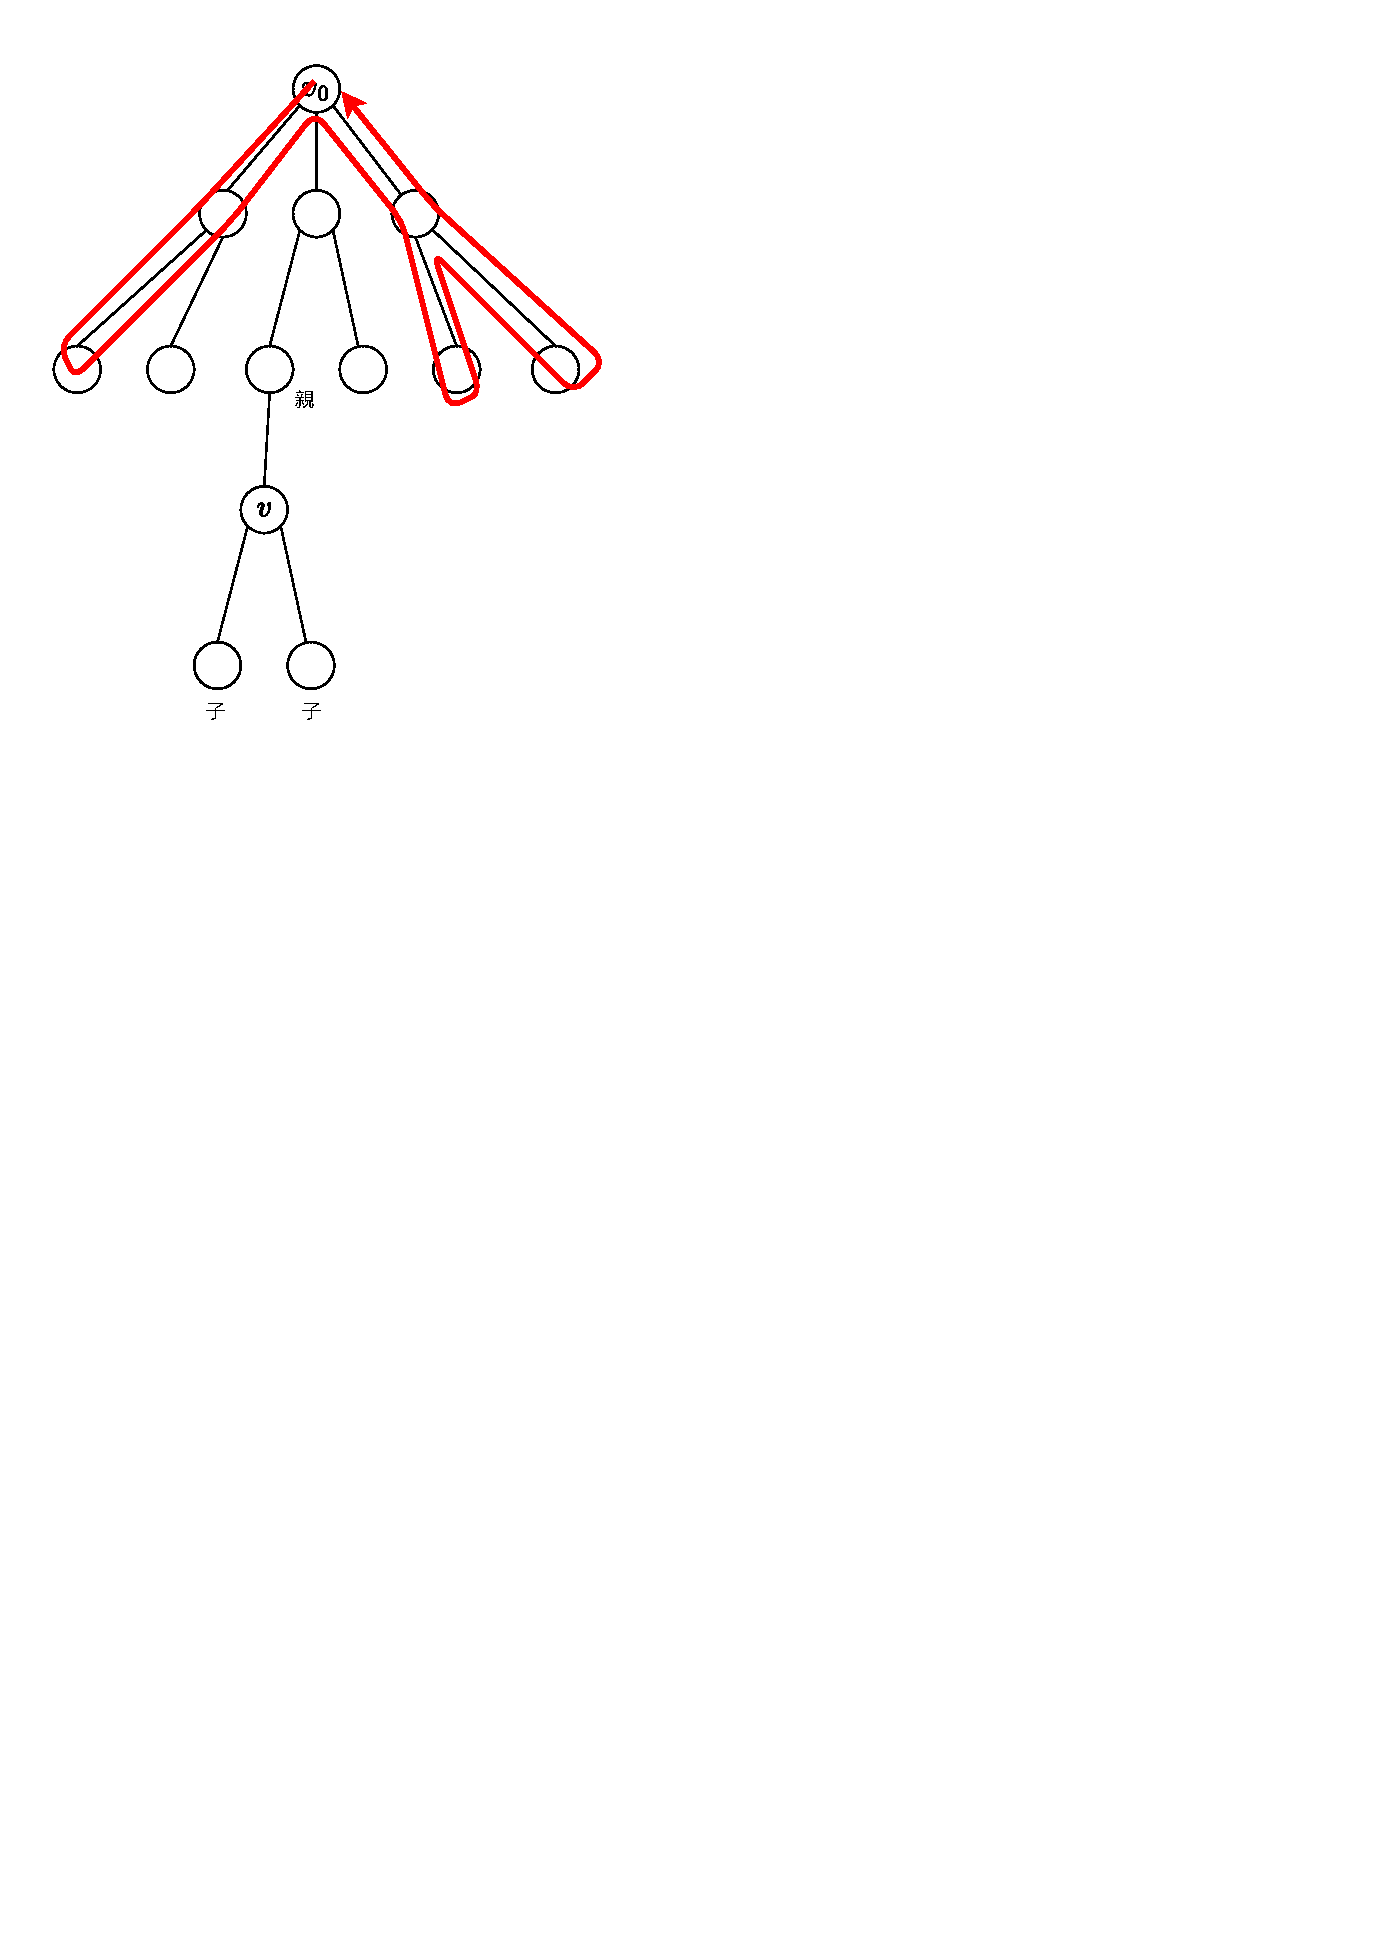
\includegraphics[width=8cm]{images/tree.pdf}
            \caption{$3$正則木$T$上の長さ$10$の閉路. 親から子への遷移と子から親への遷移を$5$回ずつ行う.}
        \end{center}
    \end{figure}

    木$T$において根を始点とする長さ$2k$の閉路$(v_0,\dots,v_{2k})$を考える (ここで$v_0=v_{2k}$).
    各$i$に対して$d_i = \mathrm{depth}(v_i)$とし, 列$(d_0,\dots,d_{2k})$を考える.
    まず$d_0=0$であり, その後は$d_{i+1} \in \cbra{d_i \pm 1}$であり, 常に非負性を保ちながら最後に$d_{2k}=0$となる.
    このような列$(d_0,\dots,d_{2k})$の総数はカタラン数と等しく, $\frac{1}{k+1}\binom{2k}{k}$に等しい.
    特に, 各$d_i - d_{i-1}$の符号を見ると$d_0 = d_{2k} = 0$より正と負がそれぞれ$k$個ずつ含まれている.

    次に, 各$(d_1,\dots,d_{2k})$に対して深さの履歴がこれと等しくなるような閉路の個数を考える.
    まず, $i=1$において, 頂点$v_0$からは子に遷移するため$v_1$の取り方は$d$通りある.
    各$i\ge 2$において, $d_i=d_{i-1}+1$ (すなわち$v_i$が$v_{i-1}$の子である)とき, $v_i$の選び方は$d-1$通りある.
    一方で親に遷移する場合はその遷移先は一意である.
    子への遷移はちょうど$k$回発生するため, 深さの履歴が与えられた$(d_1,\dots,d_{2k})$に等しくなるような閉路の個数は$d(d-1)^{k-1}$に等しい.
    従って$t_{2k} = \frac{1}{k+1}\binom{2k}{k} \cdot d(d-1)^{k-1}$を得る.

    後半の主張を証明する.
    $d$-正則グラフ$G$の頂点$u_0$を一つ固定する.
    木$T$の頂点集合を$U$, グラフ$G$の頂点集合を$V$とし,
    $N_T$の定義と同様にグラフ$G$の頂点$v \in V$に対しその$d$個の隣接頂点の集合を$N_G(v)$で表す.
    $G$から$T$への準同型写像$\phi \colon U \to V$を以下のように構成する\footnote{グラフ$G=(V,E)$から$H=(W,F)$への\emph{準同型写像 (homomorphism)}とは, 写像$\phi\colon V\to W$であって$\{u,v\}\in E\Rightarrow \{\phi(u),\phi(v)\}\in F$を満たすものである. ここでは自然に無限グラフに対してこの概念を拡張している.}:
    深さに関して帰納的に定義する.
    \begin{itemize}
        \item まず, $\phi(v_0) = u_0$とする.
              根$v_0$の子$N_T(v_0)$から$N_G(u_0)$への全単射$\phi_0$を任意に一つ選び,
              $\phi\colon N_T(v_0) \ni v' \mapsto \phi_1(v') \in N_T(u_0)$
              によって$N_T(v_0)$における$\phi$を定義する.
        \item $T$における深さ$\ell$以下の全ての頂点に対し$\phi(v)$が定義されているとする. 深さ$\ell$の各頂点$v$に対し, その親を$p$, 子を$c_1,\dots,c_{d-1}$とする. $v$とその親$p$に対しては$u\defeq \phi(v)$, $u_p\defeq \phi(p)\in U$が定義されている. このとき, 全単射$\psi\colon N_T(v)\setminus \{p\} \to N_G(u)\setminus\{u_p\}$を任意に一つ固定し, 各$\phi(c_j)$を$\psi(c_j)\in V$とする.
    \end{itemize}
    このようにして定義された写像$\phi\colon U \to V$は確かに準同型なので
    $T$の閉路$(v_0,\dots,v_{2k})$に対して$(\phi(v_0),\dots,\phi(v_{2k}))$は$G$の閉路になっている.
    さらに, $(\phi(v_0),\dots,\phi(v_{2k}))$の形になっている$G$の閉路が与えられたとき, $v_0$は一意に定まり, 以降の$v_i$は$\phi$の帰納的な定義で用いた全単射の逆写像を用いて順番に復元することができるため, $(v_0,\dots,v_{2k}) \mapsto (\phi(v_0),\dots,\phi(v_{2k}))$は単射である.
    従ってグラフ$G$に含まれるある頂点を始点とした長さ$2k$の閉路の個数は少なくとも$t_{2k}$である.
\end{proof}


\paragraph*{ラマヌジャングラフ.}
漸近的に\cref{thm:Alon Boppana}を達成するグラフを\emph{ラマヌジャングラフ (Ramanujan graph)}という.
\begin{definition}{ラマヌジャングラフ}{Ramanujan graph}
    $d$-正則グラフ$G=(V,E)$は, その単純ランダムウォークの遷移確率行列$P$の第二固有値$\lambda_2$が$\lambda_2 \le 2\sqrt{d-1}$を満たすとき, \emph{ラマヌジャングラフ (Ramanujan graph)}という.
\end{definition}

\cref{thm:Alon Boppana}を達成するグラフ列, すなわち,
次数$d$を固定したときに頂点数が増大していくグラフ列$(G_n)_{n\in\Nat}$であって各$G_n$が$d$-正則ラマヌジャングラフとなるものは存在
するだろうか?
この漸近的に最適な正則エクスパンダーグラフの構成は\citet{LPS88,Mar88}によって独立同時期に初めてその構成が与えられた.
彼らは$d-1$が$4$で割った余りが$1$となる素数であるときに$d$-正則ラマヌジャングラフの列を構成した.
なお, 「ラマヌジャングラフ」という名称は\cite{LPS88}の証明がラマヌジャン予想と呼ばれる予想に依拠しているからである
(「予想」と書いたが当時は既に解決している).
その後, \citet{Mor94}によって次数が素数べき$+1$の形であってもラマヌジャングラフが構成できることが示された.
\begin{theorem}{ラマヌジャングラフの陽な構成}{LPS Ramanujan}
    任意の素数$q$と任意の$k\in\Nat$に対して, 頂点数が発散するある$(q^k+1)$-正則ラマヌジャングラフの列が存在し, 陽に構成できる.
\end{theorem}
%また, \cite{LPS88}とは独立同時期に\citet{Mar88}もラマヌジャングラフの族を構成しているようである
%    (元論文はロシア語で書かれており, 英語に翻訳されたものもあるようなのだが見つけることはできなかった).

\paragraph*{ランダム正則グラフ.}
\citet{LPS88}やその後続研究によりラマヌジャングラフ列については様々な構成方法が知られている.
では, そもそもラマヌジャングラフは何個あるのだろうか?
$n$頂点$d$-正則グラフ全体の集合を$\calG_{n,d}$とし,
$\calG_{n,d}$から一様ランダムに選ばれたグラフ$G\sim\calG_{n,d}$を考える
($nd$は常に偶数とする).
この確率変数をランダム正則グラフという.
ランダム正則グラフは「ほぼ」ラマヌジャングラフであることが知られている
\cite{Friedman_random_regular}.
\begin{theorem}{Friedmanの定理}{random regular graph Ramanujan}
    任意の$d\ge 3$と任意の$\varepsilon > 0$に対し,
    \[ \lim_{n\to\infty}\Pr\sbra*{\lambda(P) \ge \frac{2\sqrt{d-1}}{d} + \varepsilon} = 0. \]
\end{theorem}
すなわち, ほとんど全ての定数次数正則グラフはラマヌジャングラフと同等のスペクトルを持つ.

\section{性質}
エクスパンダーグラフは固有値によって定義されるが, 様々な興味深い性質を持つことが知られている.
ここではグラフ理論的な性質, ランダムウォークに関する性質, そして擬似ランダム性について紹介する.
%
\subsection{グラフ理論的な性質}
グラフ理論的に非常に興味深い多くの性質を有する.
\todo[inline]{Cheeger, chromatic number, diameter}

\subsection{ランダムウォークの性質}
\todo[inline]{hitting time, cover time}

\subsection{擬似ランダム性(*)} \label{sec:expander pseudorandom}
この節は高次元エクスパンダーの本筋から少し外れるが,
エクスパンダーグラフの重要であることの理由の一つとしてその擬似ランダム性について概説する.

加法的組合せ論や計算量理論では\emph{擬似ランダム性 (pseudorandomness)}と呼ばれる概念が非常に重要な役割を果たしている.
\begin{definition}{分布の擬似ランダム性}{pseudorandomness}
    有限集合$\Omega$上のある分布$\mu$と関数族$\mathcal{F}=\{f\colon \Omega \to \binset\}$を考える.
    分布$\mu$は,
    任意の$f\in \mathcal{F}$に対して
    \[ \abs*{\E_{x\sim \mu} [f(x)] - \E_{y\sim U_{\Omega}}[f(y)]} \le \varepsilon\]
    を満たすとき, \emph{$\mathcal{F}$に対して$\varepsilon$-擬似ランダムである}という (ここで, $y\sim U_\Omega$とは$\Omega$上一様ランダムに$y$が選ばれたことを意味する).
\end{definition}
直感的には, 分布が擬似ランダムであるとは, その分布が任意の$f\in \mathcal{F}$を使っても一様分布と\emph{識別できない (indistinguishable)}ことを意味する.
例えば全変動距離に関する\cref{prop:dtv}では, $\mathcal{F}$を$V$上の二値関数全体 (すなわち任意の$V$の部分集合)の族としたときの識別不可能性のパラメータ$\varepsilon$が全変動距離で与えられることを意味する.
すなわち$\mu$は常に$\dtv(\mu,U_{\Omega}))$-擬似ランダムである.
関数クラス$\mathcal{F}$をより制限したときにパラメータ$\varepsilon$がどこまで小さくなるかに興味がある.

組合せ論では$\mathcal{F}$としてある特殊な関数クラスを仮定することによって\emph{組合せ論的擬似ランダム性}を定義する.
例えばグラフ理論や加法的組合せ論のコーナーストーンの一つと呼ばれるSzemerédiの正則化補題と呼ばれる結果は, 非常に大雑把に言えば
任意の密なグラフが定数個の擬似ランダムな二部グラフと疎な部分に分解できることを主張する定理である.
組合せ論的擬似ランダムネスの概念は特に加法的組合せ論において非常な協力な道具となっており,
Green--Taoの定理の証明においても重要な役割を果たしている
(驚くべきことに, 識別不可能性の枠組みでGreen--Taoの定理の証明を理解してそれを学習理論におけるブースティングの証明に応用するという研究もなされている!).

計算量理論では$\mathcal{F}$を「効率的なアルゴリズムの全体」や「素子数の少ない論理回路の全体」とすることで\emph{計算量的擬似ランダム性}を定義できる.
任意の効率的なアルゴリズムに対して一様ランダムな文字列と識別できないということは, その分布に従って生成されたメッセージを盗み見てもそこから得られる情報が何もない (ランダムな文字列を見てるのと同じ) であることから, 計算量的擬似ランダム性は暗号の計算量的安全性の定義の根幹をなすことがわかる.

エクスパンダーグラフの組合せ論的擬似ランダム性を説明する.
正則$\lambda$-エクスパンダー$G=(V,E)$を考える.
集合$\Omega=V\times V$上の分布$\mu = \mu_G$として
一様ランダムな辺$\{u,v\}\in E$を選び, $(u,v)$もしくは$(v,u)$どちらかを等確率で選んだ時の頂点対の分布とする.
すなわち,
\begin{align}
    \Pr_{(u,v)\sim \mu}\sbra*{ (u,v) = (s,t)} = \frac{\indicator{\{s,t\}\in E}}{2\abs{E}} = \frac{\indicator{\{s,t\}\in E}}{nd} \label{eq:expander mu}
\end{align}
とする.
関数族$\mathcal{F}$を
\begin{align}
    \mathcal{F} = \cbra*{ f_{S,T} \colon (s,t) \mapsto \indicator{s\in S,t\in T} \colon S,T\subseteq V}  \label{eq:expander F}
\end{align}
で定める.
%
\begin{lemma}{エクスパンダー混交補題}{expander mixing lemma}
    グラフ$G$が$n$頂点$d$-正則$\lambda$-エクスパンダーであるとき, \cref{eq:expander mu}で定義された分布$\mu$は\cref{eq:expander F}で定義された関数族$\mathcal{F}$に関して$\varepsilon$-擬似ランダムである.
    すなわち, 任意の頂点部分集合$S,T\subseteq V$に対して,
    $e(S,T) = \sum_{s\in S,t\in T} \indicator{\{s,t\} \in E}$を$S,T$間の辺の本数($S\cap T$内の辺は2回数える)とすると,
    \[
        \abs*{e(S,T) - \frac{d}{n}|S||T|} \le d\lambda\sqrt{|S||T|\rbra*{1-\frac{|S|}{n}}\rbra*{1-\frac{|T|}{n}}}.
    \]
\end{lemma}
%
グラフ$G$の隣接行列$A$を考えるとイメージしやすい.
この行列は全部で$nd$個の$1$を持っているため, 全成分の中で$1$の密度は$\frac{d}{n}$である.
ここで, 部分集合$S,T\subseteq V$に対して$A$の$S\times T$で定まる部分行列$A_{S,T}$を考える.
この行列に含まれる$1$の個数($e(S,T)$に等しい)は, $\frac{d}{n}\cdot |S||T|$に近い値となっている (\cref{fig:EML}).
\begin{figure}[htbp]
    \begin{center}
        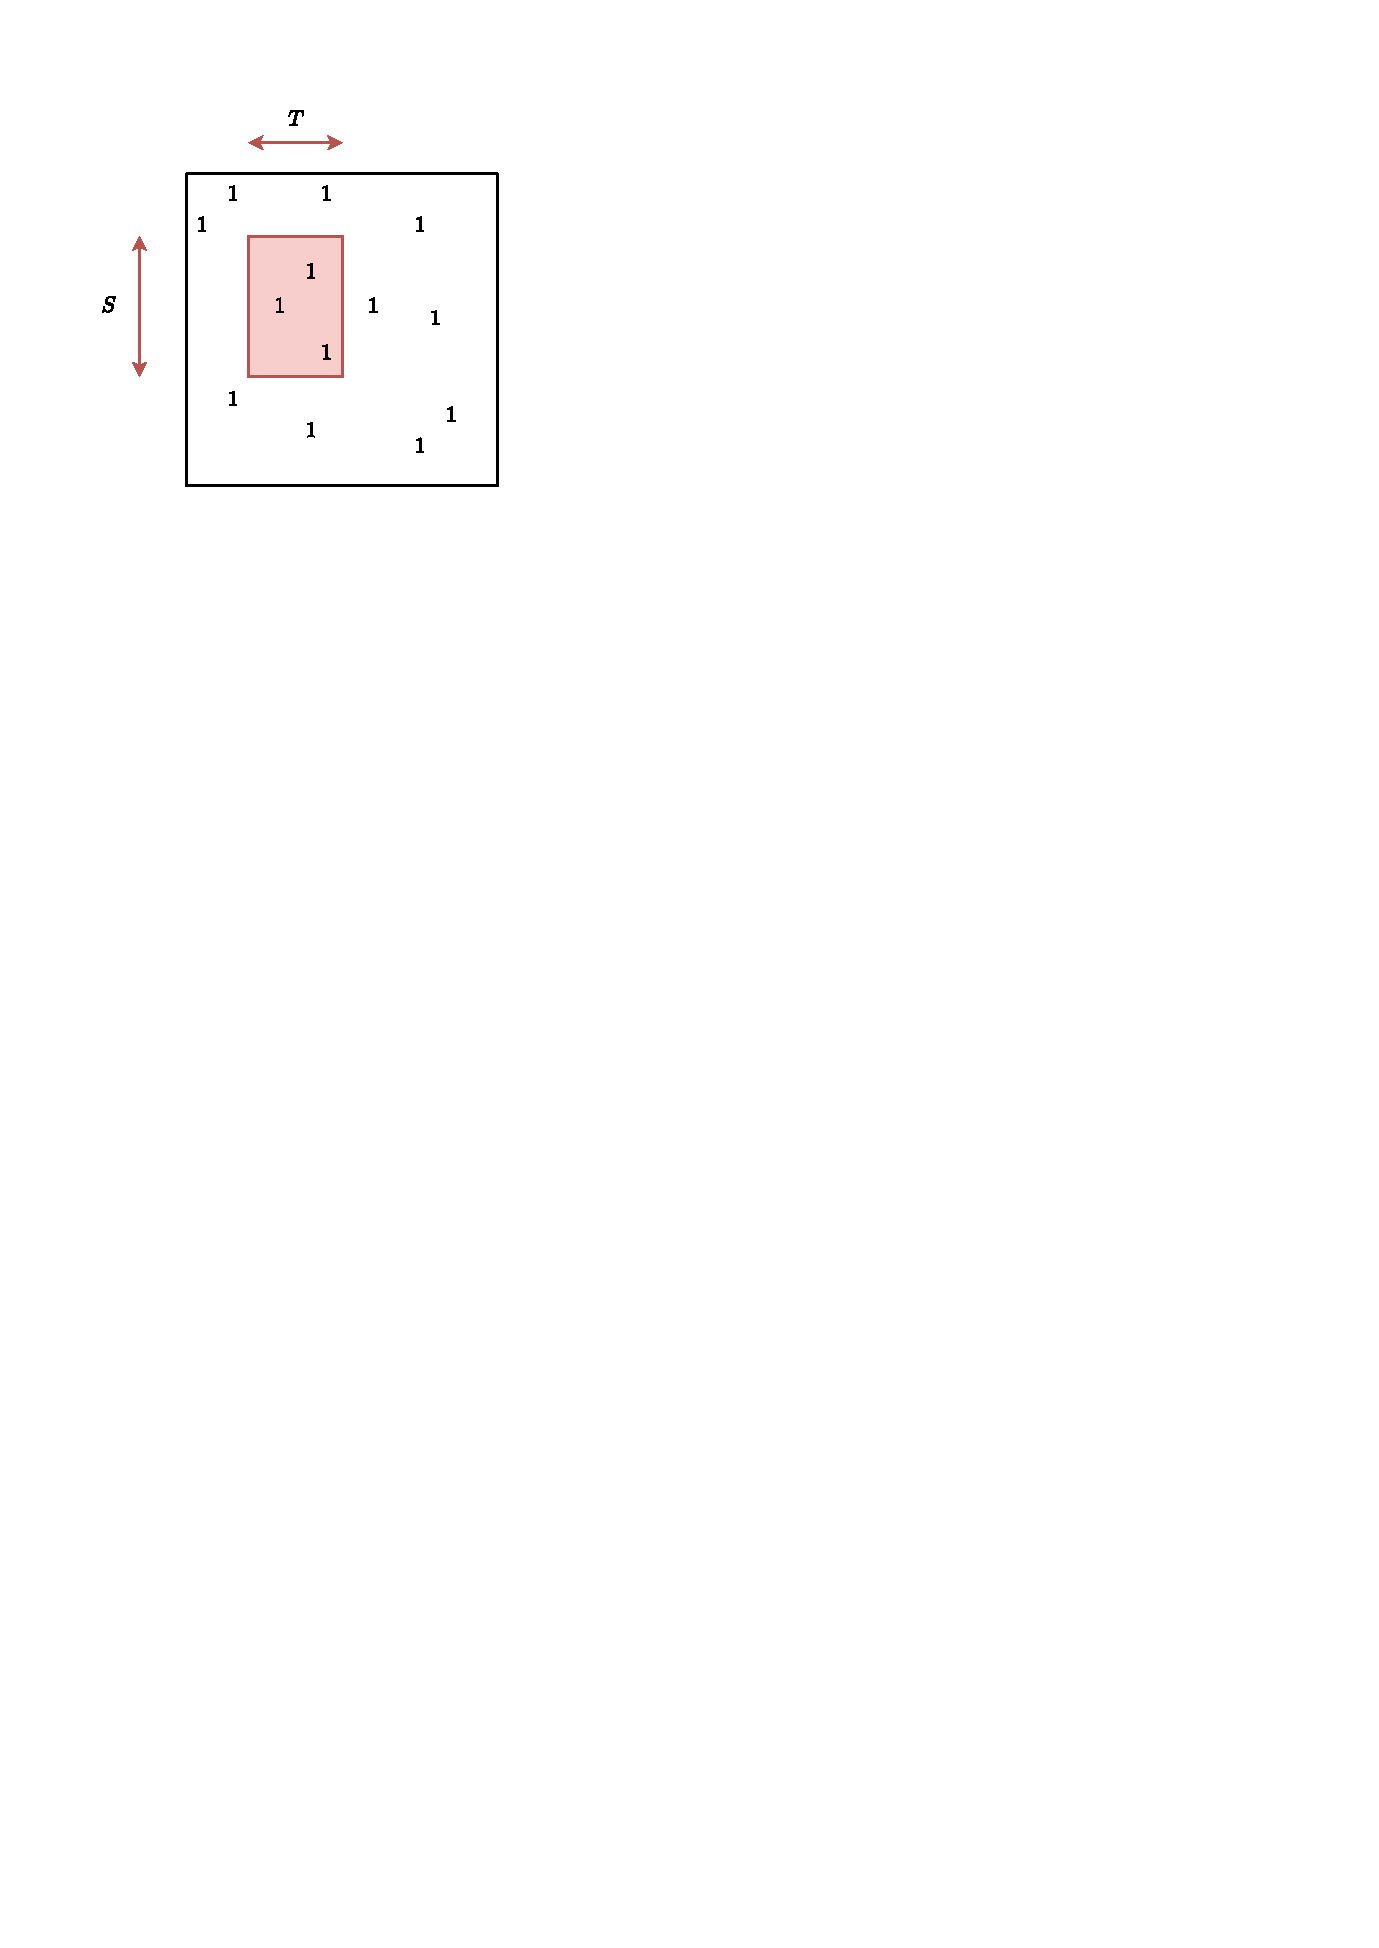
\includegraphics[width=6cm]{images/EML.pdf}
        \caption{正則グラフの隣接行列$A$を考える. このグラフがエクスパンダーならば, 頂点部分集合$S,T\subseteq V$で指定される長方形内に含まれる$1$の密度は行列全体の$1$の密度に近い値をとる. \label{fig:EML}}
    \end{center}
\end{figure}
%
\begin{proof}[\cref{lem:expander mixing lemma}の証明.]
    グラフ$G$上の単純ランダムウォーク$P$を考える.
    部分集合$S,T\subseteq V$に対し
    関数$f=\delta_S,g=\delta_T$として
    \cref{cor:general expander mixing lemma}を適用すると
    \begin{align*}
         & \piprod{f,Pg} = \frac{e(S,T)}{nd},               \\
         & \Epi f = \frac{|S|}{n},                          \\
         & \Epi [Pg] = \Epi g = \frac{|T|}{n},              \\
         & \Varpi f = \frac{|S|}{n}\rbra*{1-\frac{|S|}{n}}, \\
         & \Varpi g = \frac{|T|}{n}\rbra*{1-\frac{|T|}{n}}
    \end{align*}
    より整理すると主張を得る.
\end{proof}

\begin{exercise}{}{check}
    \cref{lem:expander mixing lemma}の証明で表した五つの等式を実際に確認せよ.
\end{exercise}


\section{エクスパンダーグラフの応用} \label{sec:expander graph application}
グラフのエクスパンダー性は組合せ論的な興味だけでなく,
理論計算機科学において多くの定理の証明の道具として非常に重要な役割を果たしている.
ここではその一端を軽く紹介する.
より詳細の議論は\cite{HLW06}を参照されたい.
%
\subsection{脱乱択化}
Albert Einsteinは「量子は確率的に振る舞う」とする量子力学の枠組みに対して懐疑的であり,
1926年にMax Bornに宛てた手紙において
\begin{quotation}
    Der Alte würfelt nicht. (神はサイコロを振らない)
\end{quotation}
と述べている.
では, アルゴリズムの神はサイコロを振るだろうか?
より具体的には, 乱択は計算能力を真に向上させるだろうか?
この哲学的な問いは90年代から今もなお計算量理論において深く研究されており,
その中心的なリーダーの一人であるAvi Wigdersonは2021年にAbel賞, 2023年にTuring賞を受賞している.

ここではエクスパンダーグラフを使って「少ないサイコロで多くのサイコロの出目をhitting性の意味で模倣できる」
という結果を紹介する.

\begin{comment}
話の分かりやすさのために多変数多項式の合同性判定(polynomial identity testing)を例に説明する.
有限体$\Fq$上の$n$変数$d$次多項式$f\colon \Fq^n\to \Fq$が恒等的に$0$かどうか (すなわち, 任意の$x\in\Real^n$に対し$f(x)=0$か否か) を判定したい\footnote{多項式合同性判定は二つの多項式$f,g$が恒等的に同じかどうかを判定する問題だが, $f-g$を考えればこの問題に帰着できる.}.
ただし有限体$\Fq$のサイズ$q$は十分大きく, 特に$\Fq>2d$を仮定する.
また, ここでは多項式$f$の次数をいわゆる全次数(total degree)で定義する.
すなわち$f(x_1,\dots,x_n)$に対しその次数$\deg f$を一変数多項式$x \mapsto f(x,\dots,x)$の最大次数として定義する.
関数$f$は\emph{オラクル}として与えられると仮定する.
すなわち, 「$x\in\Fq^n$に対して$f(x)$は何ですか?」と質問し, その答えを得ることができる.
できるだけ少ない回数の質問で$f$と$g$が恒等的に同じかどうかを判定するにはどうすればよいか?

この問題はランダムネスを許せば効率的に解ける.
次の補題を証明する.
\begin{lemma}{Schwartz--Zippelの補題}{Schwartz--Zippel}
    有限体$\Fq$上の$n$変数$d$次多項式$f \colon \Fq^n \to \Fq$が非ゼロ (ある$x\in\Fq^n$が存在して$f(x)\neq 0$) ならば,
    \[ \Pr_{x \sim \Fq^n} \sbra*{ f(x) = 0} \le \frac{d}{q}. \]
\end{lemma}
従って, 例えば$q \ge 2d$ならば, 一様ランダムな$x\sim\Fq^n$に対して$f(x)$が非ゼロかどうかを確認すれば確率$1/2$で正しくこの問題を解ける.

この乱択アルゴリズムは$x\sim\Fq^n$を乱択しているため, $n\log_q 2$ビットのランダムネスを用いている.
実は, エクスパンダーグラフを用いることでこのランダムビットの長さを減らすことができる.

\end{comment}

\subsection{誤り訂正符号}
\emph{誤り訂正符号(error-correcting code)}または単に\emph{符号(code)}とは文字列に冗長性を持たせることでノイズに対する頑健性を与える手法である.
数学的には符号はビット列の集合$\Code\subseteq\mathbb{F}_2^n$であり, その元$f\in\Code$を\emph{符号語(codeword)}と呼ぶ\footnote{文脈によってはビット列の代わりに有限集合$\Sigma$に対して$\Code\subseteq\Sigma^n$を符号と定義することもある. 実際には計算機上では$\Sigma$の元を$\lceil\log_2 |\Sigma|\rceil$ ビットで表すため$\Sigma=\mathbb{F}_2$とすることが多い.}.
ここで$n$を符号$\Code$の\emph{符号長(code length}と呼ぶ.
符号には, 任意の相異なる二つの符号語が互いにハミング距離の意味で離れていることが望まれる.
形式的には, 正規化されたハミング距離$\dist(f,g)=n^{-1}\sum_{i\in[n]}\indicator{f(i)\neq g(i)}=\Pr_{i\sim[n]}[f(i)\neq g(i)]$を考え, $\min_{f\neq g\in\Code}\dist(f,g)$を符号$\mathcal{C}$の\emph{距離(distance)}という.
文字列$f\in\mathbb{F}_2^n$と$\Code\subseteq\mathbb{F}_2^n$に対して$\dist(f,\Code)=\min_{w\in\Code}\dist(f,w)$
を$f$の$\Code$への距離とする.


符号$\Code\subseteq\mathbb{F}_2^n$が線形部分空間となるとき, 符号$\Code$を\emph{線形符号(linear code)}と呼ぶ.
文脈によっては線形符号のことを単に符号と呼ぶこともあり,
本講義も以降は特に断りのない限りこの慣習に従う.
すなわち符号と言えばそれは線形部分空間を意味する.
符号長$n$, ランク$k$の線形符号に対し,
$k/n$をその符号の\emph{レート(rate)}と呼ぶ.
直感的には符号のレートはその符号が空間$\mathbb{F}_2^n$内でどれほど密に充填しているかを表すため,
符号のレートと距離にはトレードオフがある.
線形符号$\Code$の距離は最小ハミング重みを持つ非ゼロの符号語によって与えられることに注意されたい.

ここでは, ケイリーグラフ (\cref{def:Cayley graph}) を用いて構成される符号を紹介する.
\begin{definition}{ケイリーエクスパンダー符号}{Cayley expander code}
    ケイリーグラフ$\Cay(A,G)=(V,E)$と符号$\Code_A\subseteq\mathbb{F}_2^A$を考える.
    頂点$g\in V$と関数$f\colon E \to \mathbb{F}_2$に対し, $f_g=(f(\{g,ag\}))_{a\in A}\in \mathbb{F}_2^A$と定める.
    符号$\Code_A\subseteq \mathbb{F}_2^A$に対して
    \begin{align*}
        \Code(A,G,\Code_A)=\{f\in\mathbb{F}_2^E\colon \forall g\in V, f_g \in \Code_A\}
    \end{align*}
    を\emph{ケイリーエクスパンダー符号}と呼ぶ.
\end{definition}
一般の(ケイリーグラフとは限らない)正則エクスパンダーグラフを用いて定義される\emph{エクスパンダー符号 (expander code)}が有名だが, 定義の簡潔さを優先してあえてケイリーグラフに限定したエクスパンダー符号を紹介した.
もし仮に$A$を生成系とするケイリーグラフの列$(\Cay(A,G_n))_{n\in\Nat}$と
レートと距離の良い性質をもつ一つの符号$\Code_A$があったとしよう.
すると, この一つの符号から符号の列$(\Code_n)_{n\in\Nat} \defeq (\Code(A,G_n,\Code_A))_{n\in\Nat}$を構成できる.

さらに興味深いことに, 構成に用いたケイリーグラフがエクスパンダー性を持つならば
元の符号$\Code_A$のレートと距離の性質を符号列$(\Code_n)$も受け継ぐ.
%
\begin{lemma}{}{expander code rate}
    $\Code_A$のレートが$r_A$ならば
    $\Code(A,G,\Code_A)$のレートは少なくとも$2r_A-1$である.
\end{lemma}
\begin{proof}
    符号$\Code_A\subseteq\F_2^A$のレートが$r_A$なので,
    その任意の符号語$f_0\in \Code_A$は$|A|(1-r_A)$個の線形制約を満たす.
    ケイリーエクスパンダー符号$\Code(A,G,\Code_A)$の符号語$f$は,
    全ての頂点$g\in G$に対して$f_g$が$\abs{A}(1-r_A)$個の線形制約を満たしているので,
    $f$は高々$|G||A|(1-r_A)$個の線形制約を満たしている.
    つまり$f$の自由度は少なくとも$|E|-|G||A|(1-r_A)=|E|(1-2(1-r_A))$なので,
    $\Code(A,G,\Code_A)$のレートは少なくとも$1-2(1-r_A)=2r_A-1$となる.
\end{proof}
%
\begin{lemma}{}{expander code distance}
    符号$\Code_A$の距離が$\delta_A$, ケイリーグラフ$\Cay(A,G)$が$\lambda$-エクスパンダーならば,
    ケイリーエクスパンダー符号$\Code(A,G,\Code_A)$の距離は少なくとも$\delta_A(\delta_A-\lambda)$である.
\end{lemma}
証明にはエクスパンダー混交補題からすぐに従う以下の系を用いる:
\begin{corollary}{}{EML}
    $d$-正則な$\lambda$-エクスパンダー$G=(V,E)$の頂点部分集合$S\subseteq V$が$e(S,S)\geq cd|S|$を満たす(言い換えると, 誘導部分グラフ$G[S]$の平均次数が$cd$以上)ならば, $|S|\geq (c-\lambda)n$を満たす.
\end{corollary}
%

\begin{proof}[\cref{cor:EML}の証明.]
    $S=T$として\cref{lem:expander mixing lemma}を適用すると
    \begin{align*}
        cd|S| \leq e(S,S) \leq \frac{d}{|V|}|S|^2+\lambda d |S|.
    \end{align*}
    これを解くと$|S|\geq (c-\lambda)n$を得る.
\end{proof}
%
\begin{proof}[\cref{lem:expander code distance}の証明.]
    任意の非ゼロの符号語$f\in\Code(A,G,\Code_A)$が少なくとも$\delta_A(\delta_A-\lambda)|E|$個の$1$を持つことを言えばよい.
    符号語$f\neq 0$に対し, $F=\{e\in E\colon f(e)=1\}$とし, $S=\bigcup_{e\in F}e$を$F$の辺と接続している頂点の全体とする(辺$e$を要素数$2$の頂点部分集合として見ている).
    $|F|\geq\delta_A(\delta_A-\lambda)|E|$を示せばよい.

    $\Code_A$の距離の条件より,
    各$g\in S$に対して$f_g\in\F_2^A$は少なくとも$\delta_A|A|$本の辺が接続している.
    すなわち, $\Cay(A,G)$の部分グラフ$(S,F)$の最小次数は$\delta_A|A|$を満たすので$|F|\geq \frac{\delta_A |A|}{2}|S|$.
    誘導部分グラフ$G[S]$は$(S,F)$を部分グラフとして含むので$e(S,S)\geq 2|F|$.
    さらに$(S,F)$に対する握手補題より
    \begin{align*}
        e(S,S)\geq 2|F|\geq \delta_A|A||L|.
    \end{align*}
%
    \Cref{cor:EML}より$|S|\geq (\delta_A-\lambda)|G|$なので,
    $|F|\geq \frac{\delta_A|A|}{2}|S|\geq \delta_A(\delta_A-\lambda)\frac{|G||A|}{2}=\delta_A(\delta_A-\lambda)|E|$を得る.
\end{proof}

\todo[inline]{下論文の二部エクスパンダーに基づく定義との比較}


\subsection{PCP定理}

\subsection{Goldreichの擬似乱数生成器}


%\chapter{高次元エクスパンダー概論}
高次元エクスパンダーとはグラフのエクスパンダー性を単体複体に拡張した概念である.
単体複体上では, 大域的なランダムウォークと局所的なランダムウォークの二つのタイプのランダムウォークを自然に考えることができ, これらに基づいてそれぞれ大域的なエクスパンダー性と局所的なエクスパンダー性の概念が定義できる.
端的に述べると高次元エクスパンダーの理論はこれら二つの概念がほぼ等価であることを明らかにしており, これは単体複体における「局所大域原理」\footnote{局所大域原理(local-global principle)とは整数論などで知られる不定方程式の解の存在性に関して, 局所的な情報が大域的な情報を導くという現象の総称である.}を体現しているといえる.

本チャプターではまず単体複体とその上でのランダムウォークを定義し,
これに基づいて高次元エクスパンダーの定義と重要な性質を紹介する.

\section{定義}
まずは単体複体に関する基礎的な用語を定義していく.
文脈によっては単体複体は多面体などを貼り合わせた幾何的な概念を指すこともあるが,
本講義では組合せ的ないわゆるset system (ハイパーグラフ) としての単体複体を扱う.

\begin{definition}{単体複体}{simplicial complex}
有限集合$V$と$V$の部分集合族$\F\subseteq 2^V$であって部分集合で閉じているもの(すなわち, $\sigma\subseteq \tau \in \F \Rightarrow \sigma\in \F$)の組$X=(V,\F)$を\emph{単体複体 (simplicial complex)}という.
集合族$\F$の元を\emph{面 (face)}と呼び,
面$\sigma \in \F$の\emph{次元 (dimension)}を$\dim \sigma = \abs{\sigma} - 1$とする\footnote{特に, 空集合$\emptyset \in \F$の次元は$-1$である.}.
単体複体$X$の次元を$\dim X = \max\cbra{\dim \sigma \colon \sigma \in \F}$とする.

次元$d$の単体複体$X$は(包含関係に関して)極大な面の次元が全て$d$に等しいとき, \emph{純粋 (pure)}であるという.
整数$-1 \le k \le \dim X$に対し$X(k) = \cbra*{\sigma \in \F\colon \dim \sigma = k }$とする.
特に断りのない限り, $X(0)=V$を仮定する
(そうでなければ$V$として$V=X(0)$とした単体複体を考える).
\end{definition}
面の次元の概念は単体複体の幾何的な表現に由来する.
このイメージになぞらえて,
次元$0$の面を\emph{頂点 (vertex)}, 次元$1$の面を\emph{辺 (edge)}と呼ぶことがある.
次元$2$以上の任意の単体複体$X$に対して$(X(0),X(1))$はグラフである.

\paragraph*{例1.}
グラフ$G=(V,E)$に対し, 空集合, $V$, $E$からなる部分集合族
$\F = \{\emptyset\} \cup \cbra*{\{v\}\colon v \in V} \cup E$考えると,
$(V,\F)$は単体複体である.

\paragraph*{例2.}
有限集合$V$に対し,
$\F = \binom{V}{\le k} \defeq \cbra*{ \sigma \subseteq V \colon |\sigma|\le k}$としたとき, $(V,\mathcal{F})$は純粋な$(k+1)$-次元の単体複体である.

\paragraph*{例3.}
閉路を含まないグラフを\emph{森 (forest)}といい, 連結な森を\emph{木 (tree)}という.
連結グラフ$G$の部分グラフであって木であるものを\emph{全域木 (spanning tree)}という (cf. \cref{def:graph}).
グラフ$G=(V,E)$に対し,
森であるような部分グラフの辺集合からなる集合族$\F\subseteq 2^E$は単体複体である.
すなわち,
\begin{align*}
    \F = \cbra*{ F \subseteq E \colon \text{部分グラフ$(V,F)$は森}}
\end{align*}
に対して$(E,\F)$は単体複体である.
簡単のため$G$を連結グラフであるとすると, $(E,\F)$の極大面は$G$の全域木に対応し, その次元は$n-2$に等しい.
すなわち$(E,\F)$は純粋な$(n-2)$-次元単体複体である.

なお, グラフ$G$が連結でない場合, 異なる連結成分に属する二頂点$u,v$を縮約し一つの頂点として扱うことによって$(V,\F)$の構造を変えないまま連結成分数を減らすことができるので, 連結性を仮定しても一般性を失わない.

\paragraph*{例4.}
実行列$A\in \Real^{n\times m}$ (ただし$m\ge n$) の行ベクトルを$\vec{a}_1,\dots,\vec{a}_n$とする.
集合$V=\{1,\dots,n\}$の部分集合族であって, 線形独立な行ベクトル集合のインデックスとなるものの全体を$\F$とする.
すなわち
\[
    \F = \cbra*{ I \subseteq V\colon (\vec{a}_i)_{i\in I}\text{は線形独立}}
\]
とすると, $(V,\F)$は純粋な単体複体であり, その次元は$A$のランク$\mathrm{rank}(A)$に対し$\mathrm{rank}(A)-1$となる.

\paragraph*{例5.}
部集合$L,R$を持つ二部グラフ$G=(V,E)$を考える.
辺部分集合$M\subseteq E$は, 部分グラフ$(V,M)$の全ての頂点の次数が高々$1$であるとき\emph{マッチング (matching)}という.
マッチング$M$の部分集合$M'\subseteq M$もまたマッチングであるため,
グラフ$G$のマッチング全体からなる辺部分集合族$\F\subseteq 2^E$に対し, $(E,\F)$は単体複体である.
一般に極大マッチングのサイズは異なる場合があるのでこの単体複体は純粋ではない (\cref{fig:matching}).
\begin{figure}[htbp]
    \begin{center}
        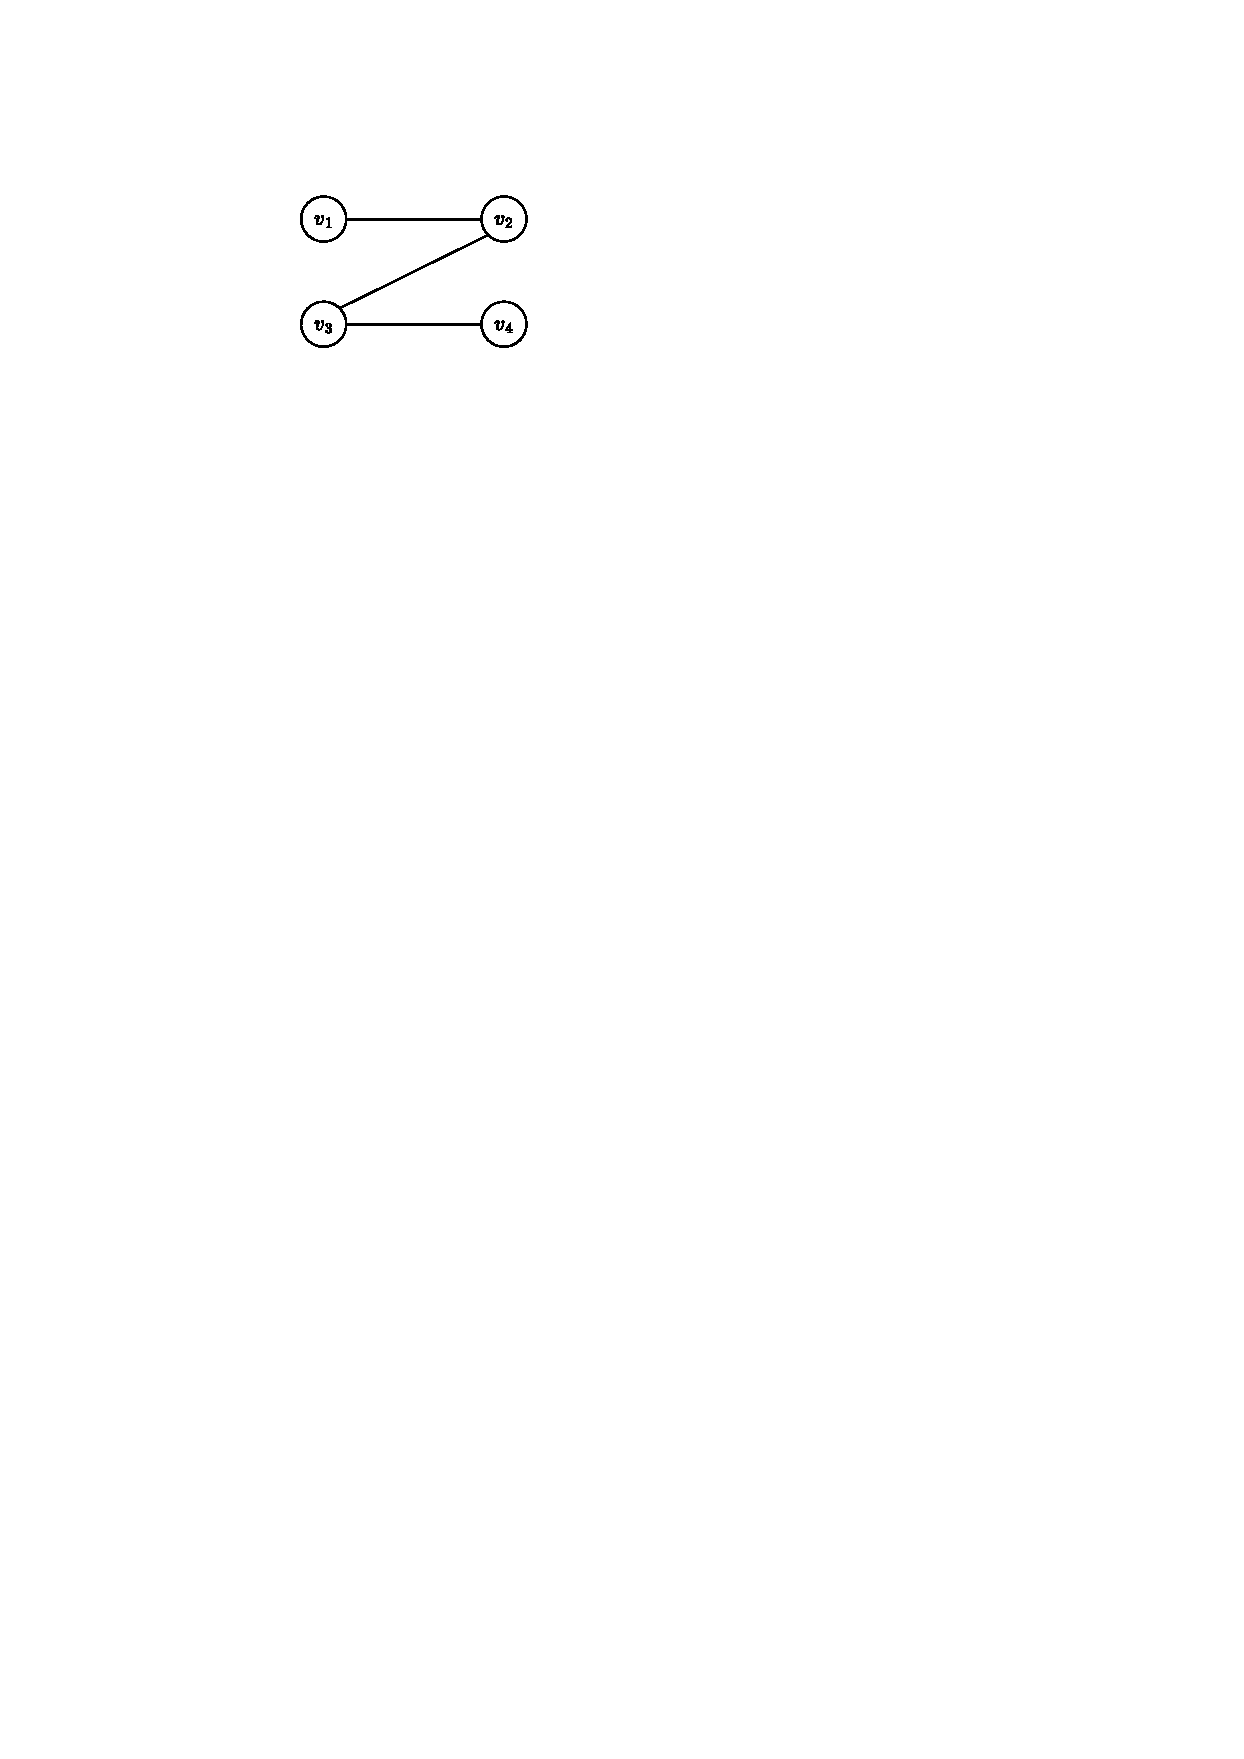
\includegraphics[width=5cm]{images/matching.pdf}
    \end{center}
    \caption{マッチング$M_1=\{v_1,v_2\},\{v_3,v_4\}\}$と$M_2=\{\{v_2,v_3\}\}$はどちらも極大である. \label{fig:matching}}
\end{figure}

\paragraph*{例6.}
グラフ$G=(V,E)$の頂点部分集合$U\subseteq V$は, $U$に属する任意の二頂点間に辺がある(すなわち$\binom{U}{2}\subseteq E$)とき, \emph{クリーク (clique)}\footnote{cliqueとは派閥を意味する英単語である.}という.
特に, 単一頂点からなる集合$\{u\}$や$\emptyset$もクリークである.
クリークの部分集合もまたクリークなので,
グラフ$G$の全てのクリークからなる頂点集合族を$\F$とすると, $(V,\F)$は単体複体である.

\begin{definition}{リンクとスケルトン}{link and skelton}
    単体複体$X=(V,\F)$を考える.
    面$\sigma \in \F$の\emph{リンク (link)}とは単体複体$(V\setminus \sigma, \F_{\sigma})$であって集合族$\F_\sigma$が
    \[
        \F_\sigma = \cbra*{ \tau \setminus \sigma \colon \sigma \subseteq \tau \in \F }
    \]
    で与えられるものである.
    次元$k$以下の面の集合
    \[
        \F_k = \cbra*{ \sigma \in \F \colon \dim \sigma \le k}
    \]
    に対し$(V,\F_k)$を\emph{$k$-スケルトン ($k$-skelton)}という.
\end{definition}
面$\sigma$のリンクとは, $\sigma$をある意味で「縮約」して得られる単体複体であり, 面$\sigma$の周りの局所的な構造を表している.
例えば連結グラフ$G=(V,E)$の森の全体からなる単体複体$X=(E,\F)$を考えよう.
$\sigma\in \F$を一つ固定したとき, リンク$X_\sigma$はどのような単体複体になっているだろうか?
$X_\sigma$の全ての面は辺集合$F$を含むので, $F$に含まれる全ての頂点を縮約して得られるより小さなグラフを考え, そこから$F$の辺を除去して得られるグラフ$G'$の森全体からなる単体複体とみなせる.

%\end{definition}
\section{大域エクスパンダー性}
グラフ上のランダムウォークは頂点集合上で遷移するものを考えていたが,
単体グラフ上のランダムウォークは異なる次元の面の間で遷移するものを考える.
具体的には, \cref{sec:graph up and down walk}で考えたようにある次元$i$の面から次元$i+1$の面に遷移する上昇ウォークと逆に次元$i+1$の面から次元$i$の面に遷移する下降ウォークである.
上昇ウォークと下降ウォークが互いに随伴の関係になるようにするため, 各$X(i)$上での定常分布を定義し, $X(i)$と$X(i+1)$の間で詳細釣り合い条件が満たされるように定義される.

\subsection{下降ウォークと定常分布}
まず, \cref{sec:graph up and down walk}で考えた下降ウォークを単体複体に拡張し, $X(d-1)$上では一様分布を定常分布とすることによって帰納的に各$X(i)$上での定常分布を定める.
\begin{definition}{下降ウォークと面上の定常分布}{down walk and stationary distribution}
    純粋な$d$次単体複体$X=(V,\F)$を考える.
    各$i=0,\dots,d-1$に対し
        確率行列$\Pdown_i \in [0,1]^{X(i) \times X(i-1)}$を
        \[
            \Pdown_i(\tau,\sigma) = \begin{cases}
                \frac{1}{i+1}	& \tif \sigma \subseteq \tau,\\
                0 & \totherwise
            \end{cases}
        \]
        とする.
    各$i=0,\dots,d-1$に対して, $X(i)$上の分布$\pi_i \in [0,1]^{X(i)}$を
        \begin{itemize}
        \item $i=d-1$のとき, $\pi_{d-1}$は$X(d-1)$上の一様分布. すなわち$\pi_{d-1}(\sigma) = \frac{1}{\abs{X(d-1)}}$
        \item $\pi_{i+1}$が定義されているとき, $\pi_i = \pi_{i+1}\Pdown_{i+1}$
        \end{itemize}
    で定める.
    分布$\pi_i$を($i$次の)定常分布と呼ぶ.
\end{definition}
面$\tau \in X(i+1)$に対して$\Pdown_{i+1}(\tau,\cdot)$で定まる$X(i)$上の分布は, 面$\tau$に含まれる頂点$u$を一様ランダムに選んだときの$\sigma = \tau \setminus\{u\}$の分布と等しい.
この分布は, まず一様ランダムに$X(d)$から面を選び, その中から一様ランダムに選ばれた$i+1$個の頂点からなる$X(i)$の面のなす分布である.
特に全ての$\sigma\in X(i)$に対し$\pi_i(\sigma)=0$である
(そうでなければ, $\pi_d$が一様分布であることに反する).
ある面$\tau\in X(i+1)$から分布$\Pdown_{i+1}(\tau,\cdot)$に従ってランダムに選ばれた面$\sigma$に遷移する過程を\emph{下降ウォーク (down walk)}と呼ぶ.

\subsection{上昇ウォーク}
\cref{def:down walk and stationary distribution}では次元$i$の面から次元$i-1$に遷移する下降ウォークを与えた.
同様に, 次元$i$の面から次元$i+1$の面に遷移する上昇ウォークを, $X(i)$と$X(i+1)$の間の詳細釣り合い条件が成り立つように定義する.
%
\begin{definition}{上昇ウォーク}{up walk}
    純粋な$d$次単体複体$X=(V,\F)$を考える.
    各$i=-1,\dots,d-2$に対し
        確率行列$\Pup_i \in [0,1]^{X(i) \times X(i+1)}$を
    \begin{align*}
        \Pup_i(\sigma,\tau) &= \frac{\pi_{i+1}(\tau)}{\pi_i(\sigma)}\Pdown_{i+1}(\tau,\sigma) \\
        &= \begin{cases}
            \frac{\pi_{i+1}(\tau)}{(i+1)\pi_i(\sigma)}	& \tif \sigma\subseteq \tau,\\
            0 & \totherwise
        \end{cases}
    \end{align*}
    で定める.
\end{definition}
%
二つの面集合$X(i)$と$X(i+1)$を部集合とする二部グラフを考えればわかりやすい.
それぞれの部集合には$\pi_i,\pi_{i+1}$が定常分布として付随しており,
上昇ウォーク$\Pup_i$と下降ウォーク$\Pdown_{i+1}$は詳細釣り合い条件
\[
    \forall \sigma\in X(i),\tau\in X(i+1),\,\pi_i(\sigma)\Pup_i(\sigma,\tau) = \pi_{i+1}(\tau)\Pdown_{i+1}(\tau,\sigma)
\]
を満たしている.

なお, 下降ウォーク$\Pdown_{i}$と上昇ウォーク$\Pup_i$の添字$i$は遷移の開始地点の面の次元としている.
%
    各$X(i)$に対して空間$\ell^2_{\pi_i}(X(i))$, 
    すなわち, \cref{def:naiseki}と同様にして$\Real^{X(i)}$に内積$\abra{\cdot,\cdot}_{\pi_i}$が導入された空間を定義できる.
    このとき, 
    \[\Pup_i\colon \ell^2_{\pi_{i+1}}(X(i+1)) \to \ell^2_{\pi_{i}}(X(i))\]
    と
    \[\Pdown_{i+1}\colon \ell^2_{\pi_{i}}(X(i)) \to \ell^2_{\pi_{i+1}}(X(i+1))\]
    は互いに随伴の関係にある.
    すなわち, 任意の$f\in \ell^2_{\pi_i}(X(i)),g\in \ell^2_{\pi_{i+1}}(X(i+1))$に対して
    \begin{align} \abra{\Pup_i f, g}_{\pi_{i+1}} = \abra{ f,\Pdown_{i+1}g }_{\pi_i} \label{eq:adjoint up and walk}\end{align}
    が成り立つ.
%
\begin{exercise}{}{adjoint check}
    \cref{eq:adjoint up and walk}を確認せよ.
    すなわち, \cref{def:down walk and stationary distribution}で定義された定常分布$\pi_i,\pi_{i+1}$および任意の二つの関数$f\colon X(i) \to \Real,g\colon X(i+1) \to \Real$に対して
    \[ \sum_{\sigma \in X(i)} \pi_i(\sigma) f(u) = \sum_{\tau \in X(i+1)} \pi_{i+1}(\tau) g(\tau) \]
を確認せよ.
\end{exercise}

最後に, 上昇ウォークと下降ウォークを組み合わせることによって面$X(i)$上の2種類のランダムウォークが定義できる:
\begin{definition}{上昇下降と下降上昇ウォーク}{UD and DU walk}
    \cref{def:down walk and stationary distribution}, \ref{def:up walk}と同じ設定を考える.
    \begin{align*}
        &\PUD_i \defeq  \Pup_i \Pdown_{i+1},\\
        &\PDU_i \defeq \Pdown_{i}\Pup_{i-1}
    \end{align*}
    を遷移確率行列として持つ$X(i)$上のランダムウォークをそれぞれ\emph{上昇下降ウォーク (up-down walk), 下降上昇ウォーク (down-up walk)}と呼ぶ.
    ここで, $X(-1)$上での下降上昇ウォークと$X(d-1)$上での上昇下降ウォークは定義されない.
\end{definition}
上昇下降ウォークはグラフ上の遅延単純ランダムウォークの自然な一般化になっている (\cref{sec:graph up and down walk}).
\begin{lemma}{定常分布}{UP and DU stationary distribution}
    面$X(i)$上の上昇下降ウォークと下降上昇ウォークはどちらも$\pi_i$を定常分布としてもつ.
\end{lemma}
\begin{proof}
    計算によって簡単に確認できる.
    実際,
    \begin{align*}
        &\pi_i \PUD_i = \pi_i \Pup_i \Pdown_{i+1} = \pi_{i+1} \Pdown_{i+1} = \pi_i, \\
        &\pi_i \PDU_i = \pi_i \Pdown_i \Pup_{i-1} = \pi_{i-1}\Pup_{i-1} = \pi_i
    \end{align*}
    より主張を得る.
\end{proof}
\begin{remark}{「上昇」「下降」の名称}{up and down}
    非常にややこしいのだが,
    上昇ウォークと下降ウォークの遷移確率行列と左右どちらから作用させるかによって「上昇」「下降」の意味合いが反転してしまう.
    確率行列としての上昇ウォークは$\Pup_i \in [0,1]^{X(i)\times X(i+1)}$で表せる.
    一般によくある左から作用させる作用素の感覚で考えると
    $\Pup_i\colon \Real^{X(i+1)} \to \Real^{X(i)}$
    であるので, 次元を一つ落とすように見えてしまうのである.
    下降ウォークについても同様である.
    特に上昇下降ウォーク$\PUD_i=\Pup_i\Pdown_{i+1}$を左から作用させると「次元を下げてから上げる」ものになるので, 下降上昇ウォークと混同しやすい.
    
    本講義はランダムウォークを主眼におき, 右から作用させるときの$\Pup_i,\Pdown_i$に興味があるので, 左固有値以外の文脈ではとにかくランダムウォークの遷移確率行列といえば右から作用させるものであると考えていき, 名称についても
    \cref{def:down walk and stationary distribution}, \ref{def:up walk}の呼称を採用している.
    
    そもそも, 遷移確率行列$P(u,v)$を「$u$から$v$に遷移する確率」として定義してしまったのが根本的な原因であり, 転置したものを改めて遷移確率行列と定義しなおせば解決できるのだが, ランダムウォークの文化ではもはや\cref{def:random walk}の定義が完全に主流となってしまっておりそれに反するとほとんどの参考文献が読みづらくなってしまうので従った.
    
    なお, 可逆なランダムウォーク(\cref{def:reversible})は内積$\piprod{\cdot,\cdot}$の意味で左右どちらから作用させても本質的に同じであるので左右どちらから作用させるかについてこのような煩雑な話は考えなくて良い.
\end{remark}

\section{局所エクスパンダー性}
単体複体の各リンクに対して局所的なランダムウォークを次のように定義する.
\subsection{局所的なランダムウォーク}
全てのリンクの$2$-スケルトン上での局所的な重み付きランダムウォークを考える.
重み付きランダムウォークについては\cref{def:weighted random walk}を参照されたい.
%
\begin{definition}{局所ランダムウォーク}{local random walk}
    純粋な$d$次元単体複体$X = (V,\F)$を考える.
    次元$i \le d-2$の面$\sigma \in \F$に対し,
        リンク$X_\sigma$の$2$-スケルトンを$G_\sigma = (V_\sigma,E_\sigma)$とする.
    このグラフの辺重み$w_\sigma\colon E_\sigma \to [0,1]$を
    \[ w_\sigma(e) = \pi_i(\sigma\cup e) \]
    で定め, これによって定まる$V_\sigma$上の重み付きランダムウォークを面$\sigma$に関する\emph{局所ランダムウォーク (local random walk)}と呼び\footnote{このランダムウォークの概念は高次元エクスパンダーの文脈ではほぼ必ず登場するが, 特に標準的な用語が与えられてはいないので、「局所ランダムウォーク」という用語は本講義だけの局所的なものとする.}, 遷移確率行列を$P_\sigma\in [0,1]^{V_\sigma\times V_\sigma}$とする.
\end{definition}
%
必ずしも局所ランダムウォークが既約性や非周期性を持つとは限らない(すなわち, グラフ$G_\sigma$が非連結だったり二部グラフになりうる)が,
可逆性は必ず満たすことに注意せよ.

グラフ($1$次元単体複体)だと面$\emptyset$に対する局所ランダムウォークのみ存在するが, これは上昇下降ウォーク(すなわち遅延単純ランダムウォーク)と同じである.
従って局所ランダムウォークの概念はより高次元の単体複体を考える際に意味を持つ.

%
\begin{lemma}{}{local random walk stationary distribution}
    遷移確率行列$P_\sigma$をもつ局所ランダムウォークの定常分布を$\pi_\sigma$とすると, 
\end{lemma}
%
\subsection{局所エクスパンダー}
純粋な単体複体の局所的なエクスパンダー性を定義する.
任意の面$\sigma$に対し$G_\sigma$上での局所ランダムウォークの第二固有値が小さいとき, その単体複体は局所的エクスパンダー性をもつという.
\begin{definition}{局所エクスパンダー性}{local expander}
    純粋な$d$次元単体複体$X=(V,\F)$は,
    任意の面$\sigma\in\F$に対し$\lambda_2(P)\le \lambda$を満たすとき,
    \emph{局所$\lambda$-エクスパンダー (local $\lambda$-expander)}であるという.
    より一般に, 任意の$i=-1,\dots,d-2$と任意の面$\sigma\in X(i)$に対して$\lambda_2(P_\sigma) \le \lambda_i$を満たすとき, 単体複体$X$は局所$(\lambda_{-1},\dots,\lambda_{d-2})$-エクスパンダーであるという.
\end{definition}
エクスパンダーグラフ(\cref{def:expander})と比較すると, 片側($\lambda_2$)だけの上界だけでエクスパンダー性を定義している.
これは, 単体複体上の上昇下降ウォークがグラフ上の遅延単純ランダムウォークに対応していることに起因する (遅延単純ランダムウォークの遷移確率行列は半正定値だから$\lambda_2$の上界だけあれば混交性が保証される).
%

\section{Oppenheimのトリクルダウン定理}

\section{高次元エクスパンダーの応用}
理論計算機科学における高次元エクスパンダーの応用を簡単にまとめる.
特にマトロイドに関するものは次チャプターにて解説する.
本質的には,
局所的な情報(局所ランダムウォークの混交性)が大域的な情報(上昇下降ランダムウォークの混交性)を導出するという性質が極めて重要であり,
これに基づいて誤り訂正符号などの構成がなされている.
%\chapter{マトロイド}
マトロイド(matroid)は「行列(matrix)のようなもの(-oid)」という名を冠するが,
線形代数における線型独立性をグラフの全域木などに拡張した概念である.

\section{定義}
\begin{definition}{マトロイド}{matroid}
    次の性質を持つ単体複体$(V,\F)$を\emph{マトロイド (matroid)}という:
    任意の$\sigma,\tau \in \F$に対し, $\abs{\sigma} < \abs{\tau}$ならば,
    ある$ u \in \tau \setminus \sigma$が存在して
    $\sigma \cup \cbra{u} \in \F$.
\end{definition}

\section{例}
\subsection{グラフ的マトロイド}
\subsection{線形マトロイド}
\section{モチベーション}
\subsection{組合せ最適化}
\subsection{組合せ論}
\section{基の数え上げ}
\section{Anari, Liu, Gharan, Vinzantの定理}

\printbibliography
\appendix
\chapter{付録}

\section{基本的な確率の不等式}
この節では, 証明の中で用いられる確率の不等式とその証明を述べる.
\begin{lemma}{Markovの不等式}{markov-inequality}
  任意の非負の確率変数$X$と任意の$t>0$に対し,
  \begin{align*}
    \Pr[X\ge t] \le \frac{\E[X]}{t}
  \end{align*}
  が成り立つ.
\end{lemma}

\begin{proof}
  ここでは簡単のため, $X$の台$\Omega=\supp(X)\subseteq\Real$は有限集合, すなわち$\abs{\Omega}<\infty$と仮定する\footnote{確率変数$X$のとりうる値の集合, すなわち$\qty{x\colon \Pr[X=x]>0}$を$X$の台と呼び, $\supp(X)$と表す.}.
  このとき,
  \begin{align*}
    \E[X] = \sum_{x\in \Omega} x\Pr[X=x] \ge \sum_{x\in \Omega,x\ge t} x\Pr[X=x] \ge \sum_{x\in \Omega,x\ge t} t\Pr[X=x] = t\Pr[X\ge t]
  \end{align*}
  を整理すると主張を得る.
\end{proof}

\begin{lemma}{Chebyshevの不等式}{chebyshev-inequality}
  期待値$\E[X]$と分散$\Var[X]$が存在する任意の確率変数$X$と任意の$t>0$に対し,
  \begin{align*}
    \Pr[|X-\E[X]|\ge t] \le \frac{\Var[X]}{t^2}
  \end{align*}
  が成り立つ.
\end{lemma}
\begin{proof}
  確率変数$Y=(X-\E[X])^2$は非負の確率変数であるから, これにMarkovの不等式を適用すると
  \begin{align*}
    \Pr\qty[ \abs{X - \E[X]} \ge t  ] &= \Pr\qty[ (X-\E[X])^2 \ge t^2 ] \\
    &\le \frac{\E\qty[ (X-\E[X])^2 ]}{t^2} \\
    & = \frac{\Var[X]}{t^2}
  \end{align*}
  を得る.
\end{proof}

\begin{lemma}{Paley-Zygmundの不等式}{paley-zigmund-inequality}
  非負整数値をとる任意の確率変数$X$に対し,
  \begin{align*}
    \Pr[X\ge 1] \ge \frac{\E[X]^2}{\E[X^2]}.
  \end{align*}
\end{lemma}
\begin{proof}
  非負整数値をとる確率変数$X$に対し
  \begin{align*}
    \E[X] &= \E[X\cdot \indicator{X\ge 1}] \\
    &\le \sqrt{ \E[X^2]\cdot \E[\indicator{X\ge 1}] } & & \because\text{Cauchy-Schwarzの不等式}\\
    &= \sqrt{ \E[X^2]\cdot \Pr[X\ge 1] }.
  \end{align*}
  両辺を二乗して整理すると主張を得る.  
\end{proof}
\end{document}